% Options for packages loaded elsewhere
% Options for packages loaded elsewhere
\PassOptionsToPackage{unicode}{hyperref}
\PassOptionsToPackage{hyphens}{url}
\PassOptionsToPackage{dvipsnames,svgnames,x11names}{xcolor}
%
\documentclass[
  british,
  10pt,
]{article}
\usepackage{xcolor}
\usepackage{amsmath,amssymb}
\setcounter{secnumdepth}{-\maxdimen} % remove section numbering
\usepackage{iftex}
\ifPDFTeX
  \usepackage[T1]{fontenc}
  \usepackage[utf8]{inputenc}
  \usepackage{textcomp} % provide euro and other symbols
\else % if luatex or xetex
  \usepackage{unicode-math} % this also loads fontspec
  \defaultfontfeatures{Scale=MatchLowercase}
  \defaultfontfeatures[\rmfamily]{Ligatures=TeX,Scale=1}
\fi
\usepackage{lmodern}
\ifPDFTeX\else
  % xetex/luatex font selection
\fi
% Use upquote if available, for straight quotes in verbatim environments
\IfFileExists{upquote.sty}{\usepackage{upquote}}{}
\IfFileExists{microtype.sty}{% use microtype if available
  \usepackage[]{microtype}
  \UseMicrotypeSet[protrusion]{basicmath} % disable protrusion for tt fonts
}{}
\makeatletter
\@ifundefined{KOMAClassName}{% if non-KOMA class
  \IfFileExists{parskip.sty}{%
    \usepackage{parskip}
  }{% else
    \setlength{\parindent}{0pt}
    \setlength{\parskip}{6pt plus 2pt minus 1pt}}
}{% if KOMA class
  \KOMAoptions{parskip=half}}
\makeatother
% Make \paragraph and \subparagraph free-standing
\makeatletter
\ifx\paragraph\undefined\else
  \let\oldparagraph\paragraph
  \renewcommand{\paragraph}{
    \@ifstar
      \xxxParagraphStar
      \xxxParagraphNoStar
  }
  \newcommand{\xxxParagraphStar}[1]{\oldparagraph*{#1}\mbox{}}
  \newcommand{\xxxParagraphNoStar}[1]{\oldparagraph{#1}\mbox{}}
\fi
\ifx\subparagraph\undefined\else
  \let\oldsubparagraph\subparagraph
  \renewcommand{\subparagraph}{
    \@ifstar
      \xxxSubParagraphStar
      \xxxSubParagraphNoStar
  }
  \newcommand{\xxxSubParagraphStar}[1]{\oldsubparagraph*{#1}\mbox{}}
  \newcommand{\xxxSubParagraphNoStar}[1]{\oldsubparagraph{#1}\mbox{}}
\fi
\makeatother

\usepackage{color}
\usepackage{fancyvrb}
\newcommand{\VerbBar}{|}
\newcommand{\VERB}{\Verb[commandchars=\\\{\}]}
\DefineVerbatimEnvironment{Highlighting}{Verbatim}{commandchars=\\\{\}}
% Add ',fontsize=\small' for more characters per line
\usepackage{framed}
\definecolor{shadecolor}{RGB}{248,248,248}
\newenvironment{Shaded}{\begin{snugshade}}{\end{snugshade}}
\newcommand{\AlertTok}[1]{\textcolor[rgb]{0.94,0.16,0.16}{#1}}
\newcommand{\AnnotationTok}[1]{\textcolor[rgb]{0.56,0.35,0.01}{\textbf{\textit{#1}}}}
\newcommand{\AttributeTok}[1]{\textcolor[rgb]{0.13,0.29,0.53}{#1}}
\newcommand{\BaseNTok}[1]{\textcolor[rgb]{0.00,0.00,0.81}{#1}}
\newcommand{\BuiltInTok}[1]{#1}
\newcommand{\CharTok}[1]{\textcolor[rgb]{0.31,0.60,0.02}{#1}}
\newcommand{\CommentTok}[1]{\textcolor[rgb]{0.56,0.35,0.01}{\textit{#1}}}
\newcommand{\CommentVarTok}[1]{\textcolor[rgb]{0.56,0.35,0.01}{\textbf{\textit{#1}}}}
\newcommand{\ConstantTok}[1]{\textcolor[rgb]{0.56,0.35,0.01}{#1}}
\newcommand{\ControlFlowTok}[1]{\textcolor[rgb]{0.13,0.29,0.53}{\textbf{#1}}}
\newcommand{\DataTypeTok}[1]{\textcolor[rgb]{0.13,0.29,0.53}{#1}}
\newcommand{\DecValTok}[1]{\textcolor[rgb]{0.00,0.00,0.81}{#1}}
\newcommand{\DocumentationTok}[1]{\textcolor[rgb]{0.56,0.35,0.01}{\textbf{\textit{#1}}}}
\newcommand{\ErrorTok}[1]{\textcolor[rgb]{0.64,0.00,0.00}{\textbf{#1}}}
\newcommand{\ExtensionTok}[1]{#1}
\newcommand{\FloatTok}[1]{\textcolor[rgb]{0.00,0.00,0.81}{#1}}
\newcommand{\FunctionTok}[1]{\textcolor[rgb]{0.13,0.29,0.53}{\textbf{#1}}}
\newcommand{\ImportTok}[1]{#1}
\newcommand{\InformationTok}[1]{\textcolor[rgb]{0.56,0.35,0.01}{\textbf{\textit{#1}}}}
\newcommand{\KeywordTok}[1]{\textcolor[rgb]{0.13,0.29,0.53}{\textbf{#1}}}
\newcommand{\NormalTok}[1]{#1}
\newcommand{\OperatorTok}[1]{\textcolor[rgb]{0.81,0.36,0.00}{\textbf{#1}}}
\newcommand{\OtherTok}[1]{\textcolor[rgb]{0.56,0.35,0.01}{#1}}
\newcommand{\PreprocessorTok}[1]{\textcolor[rgb]{0.56,0.35,0.01}{\textit{#1}}}
\newcommand{\RegionMarkerTok}[1]{#1}
\newcommand{\SpecialCharTok}[1]{\textcolor[rgb]{0.81,0.36,0.00}{\textbf{#1}}}
\newcommand{\SpecialStringTok}[1]{\textcolor[rgb]{0.31,0.60,0.02}{#1}}
\newcommand{\StringTok}[1]{\textcolor[rgb]{0.31,0.60,0.02}{#1}}
\newcommand{\VariableTok}[1]{\textcolor[rgb]{0.00,0.00,0.00}{#1}}
\newcommand{\VerbatimStringTok}[1]{\textcolor[rgb]{0.31,0.60,0.02}{#1}}
\newcommand{\WarningTok}[1]{\textcolor[rgb]{0.56,0.35,0.01}{\textbf{\textit{#1}}}}

\usepackage{longtable,booktabs,array}
\usepackage{calc} % for calculating minipage widths
% Correct order of tables after \paragraph or \subparagraph
\usepackage{etoolbox}
\makeatletter
\patchcmd\longtable{\par}{\if@noskipsec\mbox{}\fi\par}{}{}
\makeatother
% Allow footnotes in longtable head/foot
\IfFileExists{footnotehyper.sty}{\usepackage{footnotehyper}}{\usepackage{footnote}}
\makesavenoteenv{longtable}
\usepackage{graphicx}
\makeatletter
\newsavebox\pandoc@box
\newcommand*\pandocbounded[1]{% scales image to fit in text height/width
  \sbox\pandoc@box{#1}%
  \Gscale@div\@tempa{\textheight}{\dimexpr\ht\pandoc@box+\dp\pandoc@box\relax}%
  \Gscale@div\@tempb{\linewidth}{\wd\pandoc@box}%
  \ifdim\@tempb\p@<\@tempa\p@\let\@tempa\@tempb\fi% select the smaller of both
  \ifdim\@tempa\p@<\p@\scalebox{\@tempa}{\usebox\pandoc@box}%
  \else\usebox{\pandoc@box}%
  \fi%
}
% Set default figure placement to htbp
\def\fps@figure{htbp}
\makeatother



\ifLuaTeX
\usepackage[bidi=basic]{babel}
\else
\usepackage[bidi=default]{babel}
\fi
% get rid of language-specific shorthands (see #6817):
\let\LanguageShortHands\languageshorthands
\def\languageshorthands#1{}
\ifLuaTeX
  \usepackage[english]{selnolig} % disable illegal ligatures
\fi


\setlength{\emergencystretch}{3em} % prevent overfull lines

\providecommand{\tightlist}{%
  \setlength{\itemsep}{0pt}\setlength{\parskip}{0pt}}



 


% preamble.tex

% --- Page Layout and Geometry ---
\usepackage[a4paper, left=25mm, right=25mm, top=25mm, bottom=25mm]{geometry}

% --- Typography Settings ---

\frenchspacing                % Single space after periods
\tolerance=400                % Default is 200; higher values allow more relaxed line-breaking.
\emergencystretch=3em         % Adds additional space to help line-breaking.
\hyphenpenalty=20             % Default is 50; lower values encourage hyphenation.

% --- Microtype Settings (adjust only if needed) ---

\usepackage{microtype}        % Improves typography
\microtypesetup{
   tracking = true,
   protrusion=true,
   expansion=true,
   factor = 1100,
   stretch = 15,
   shrink = 15
}

% --- Shrink syntax-highlighted code block font size ---
\let\oldtexttt\texttt
\renewcommand{\texttt}[1]{\oldtexttt{\small #1}}

\usepackage{etoolbox}
\AtBeginEnvironment{Highlighting}{\footnotesize}

% --- Shrink code output ---%
\usepackage{etoolbox}
\AtBeginEnvironment{verbatim}{\footnotesize}

\usepackage{etoolbox}
\AtBeginEnvironment{Shaded}{\footnotesize}
\makeatletter
\@ifpackageloaded{caption}{}{\usepackage{caption}}
\AtBeginDocument{%
\ifdefined\contentsname
  \renewcommand*\contentsname{Table of contents}
\else
  \newcommand\contentsname{Table of contents}
\fi
\ifdefined\listfigurename
  \renewcommand*\listfigurename{List of Figures}
\else
  \newcommand\listfigurename{List of Figures}
\fi
\ifdefined\listtablename
  \renewcommand*\listtablename{List of Tables}
\else
  \newcommand\listtablename{List of Tables}
\fi
\ifdefined\figurename
  \renewcommand*\figurename{Figure}
\else
  \newcommand\figurename{Figure}
\fi
\ifdefined\tablename
  \renewcommand*\tablename{Table}
\else
  \newcommand\tablename{Table}
\fi
}
\@ifpackageloaded{float}{}{\usepackage{float}}
\floatstyle{ruled}
\@ifundefined{c@chapter}{\newfloat{codelisting}{h}{lop}}{\newfloat{codelisting}{h}{lop}[chapter]}
\floatname{codelisting}{Listing}
\newcommand*\listoflistings{\listof{codelisting}{List of Listings}}
\makeatother
\makeatletter
\makeatother
\makeatletter
\@ifpackageloaded{caption}{}{\usepackage{caption}}
\@ifpackageloaded{subcaption}{}{\usepackage{subcaption}}
\makeatother
\makeatletter
\@ifpackageloaded{sidenotes}{}{\usepackage{sidenotes}}
\@ifpackageloaded{marginnote}{}{\usepackage{marginnote}}
\makeatother
\usepackage{bookmark}
\IfFileExists{xurl.sty}{\usepackage{xurl}}{} % add URL line breaks if available
\urlstyle{same}
\hypersetup{
  pdftitle={BCB744: Biostatistics R Exam},
  pdfauthor={Smit, A. J.},
  pdflang={en-GB},
  colorlinks=true,
  linkcolor={blue},
  filecolor={blue},
  citecolor={blue},
  urlcolor={blue},
  pdfcreator={LaTeX via pandoc}}


\title{BCB744: Biostatistics R Exam}
\author{Smit, A. J.}
\date{2025-05-30}
\begin{document}
\maketitle


\section{About the Exam}\label{about-the-exam}

The Biostatistics Exam will start at 8:30 on 30 May, 2025 and you have
until 8:30 on 31 May, 2025 to complete it. This exam may be conducted
anywhere in the world, and it will contribute 70\% of the final
assessment marks for the Biostatistics component of the BCB744 module.

\section{Assessment Criteria}\label{assessment-criteria}

Your responses will be evaluated based on the following criteria:

\begin{enumerate}
\def\labelenumi{\arabic{enumi}.}
\tightlist
\item
  \textbf{Technical Accuracy (50\%)}

  \begin{itemize}
  \tightlist
  \item
    Correct application of data analyses and statistical methods.
    Statistical tests should address the hypotheses within what was
    taught in BCB744. The assessor recognises that students will not
    have access to the level of statistical knowledge and experience a
    research statistician might have. For example, in places, linear
    mixed models might be more suited to the questions, but students
    only were taught the basics about ANOVA and simple linear model
    (relatively simple designs). When non-parametric alternatives are
    required, I'll assign marks to the any statement that suggests the
    correct test to use, but not actually marks the execution of those
    tests.
  \item
    Use of appropriate R packages, functions, and syntax (code style and
    liberal commenting)
  \item
    Appropriate choice and justification of techniques, including due
    consideration for the assumptions of the methods used
  \item
    Accurate calculations and results interpretation, down to small
    details such as how many decimal places to use
  \end{itemize}
\item
  \textbf{Depth of Analysis (20\%)}

  \begin{itemize}
  \tightlist
  \item
    Comprehensive exploration of the problem
  \item
    Insightful interpretation of results
  \item
    Consideration of shortfalls in the analysis (due to data
    limitations, assumptions, etc.), and suggestions for improvement
  \item
    Application of out-of-the-box thinking to the problem
  \end{itemize}
\item
  \textbf{Clarity and Communication (20\%)}

  \begin{itemize}
  \tightlist
  \item
    Logical organisation of ideas, including clear section headings and
    subheadings
  \item
    Clear and concise explanations at each stage of the analysis
  \item
    Effective use of publication quality visualisations where
    appropriate, including all necessary annotations
  \item
    Communication of results in a way that is appropriate for a
    scientific audience (e.g.~a journal article)
  \end{itemize}
\item
  \textbf{Critical Thinking Shown in Final Conclusion/Synopsis (10\%)}

  \begin{itemize}
  \tightlist
  \item
    Discussion of the findings in the context of the problem (add
    ecological context, etc., as you deem necessary)
  \item
    Identification of limitations
  \item
    Discussion of assumptions
  \item
    Consideration of broader implications
  \end{itemize}
\end{enumerate}

\textbf{\emph{General Notes to Assessor (applies to all tasks):}}

\begin{itemize}
\tightlist
\item
  Heavily penalise untidy formatting, good document structure according
  to logical headings and heading hierarchies, excessive output of long,
  unnecessary data printouts (other than the obvious and required used
  of \texttt{head()}, \texttt{tail()}, \texttt{glimpse()}, and
  \texttt{summary()}) that serve no purpose {[}-15\%{]}.
\item
  Answers where the code gives error messages (it fails to run to
  provide the required output) get 0 for that question.
\item
  Where students write long-form text feedback/answers within code
  blocks, where it should have been more appropriately placed within the
  markdown text between code blocks and presented in full sentences,
  should be penalised {[}-10\% for each question where this occurs{]}.
\item
  Text answers written as bullet points and which lacks detailed
  explanatory power gets penalised {[}-10\%{]}.
\item
  Untidy presentation and formatting that fails to resemble my model
  answers (below) penalised {[}-15\%{]}.
\end{itemize}

{The marks indicated for each task reflect the relative weight and
expected depth of your response. Focus on demonstrating both technical
proficiency and conceptual understanding in your answers.}

Please refer to the
\href{https://tangledbank.netlify.app/BCB744/BCB744_index.html\#sec-policy}{Assessment
Policy} for more information on the test format and rules.

\section{Instructions}\label{instructions}

{\textbf{This is the open book assessment.}}

You must address all tasks in the allocated time of 24-hr. Please submit
your answers in a neatly formatted .html document (produced from a
Quarto document in RStudio) and submit it to the iKamva platform.

Clearly structure the document according to the task numbers, i.e., use
appropriately hierarchical headings, subheadings, and sub-subheadings to
structure your document logically.

Naming convention:
\texttt{BCB744\_Biostatistics\_Prac\_Exam\_YourSurname.html}

\section{Background}\label{background}

These data represent the aerial cover of kelp canopy in South Africa, as
measured by Landsat satellites, for the period 1984 to 2024 at a
quarterly interval. The intention is to understand the spatio-temporal
patterns in kelp canopy cover and to explore how these patterns may be
related to coastal sections and biogeographical provinces.

You are provided with two datasets at the Google Drive link emailed to
you:

\begin{enumerate}
\def\labelenumi{\arabic{enumi}.}
\tightlist
\item
  A table of 58 coastal sections (\texttt{58\_sections.csv}) that
  partitions the South African coastline into approximately 50 km
  intervals. Each section is defined by a single coordinate point
  (latitude, longitude) representing the boundary of the section.
\item
  A table of the biogeographical provinces (\texttt{bioregions.csv})
  that the 58 coastal sections fall within. There is one row for each of
  the 58 sections. For this exercise, the biogeographical classification
  by Professor John Bolton is of interest.
\item
  A netCDF file (\texttt{kelpCanopyFromLandsat\_SouthAfrica\_v04.nc}) of
  kelp sampling locations and aerial cover data -- these are presented
  as various variables at grid points across time.
\end{enumerate}

\subsection{Task 1: Initial Processing}\label{task-1-initial-processing}

\begin{itemize}
\tightlist
\item
  \textbf{{[}Task Weight: 10\%{]}}
\item
  \textbf{{[}Components (1) and (2) marked on a 0--100 scale, then
  scaled to equal proportions of the Task Weight of 10\%{]}}
\end{itemize}

You are provided with a NetCDF file that contains satellite-derived
measurements of kelp canopy area across the South African coastline from
1984 to 2024, sampled quarterly. Each observation corresponds to a grid
cell at a specific time point.

\begin{enumerate}
\def\labelenumi{\arabic{enumi}.}
\tightlist
\item
  Read the kelp canopy area, time, location (latitude/longitude), and
  satellite pass data from the NetCDF file. Once unpacked, it contains
  over 5 million rows. Your processing workflow will include:
\end{enumerate}

\begin{itemize}
\tightlist
\item
  extracting data from the netCDF file where \texttt{area} and
  \texttt{passes} are variables defined over 3D space
  (\texttt{longitude}, \texttt{latitude}, and \texttt{time}); and
\item
  using functions such as \texttt{tidync::hyper\_tibble()} or
  \texttt{ncdf4::ncvar\_get()} to read these values.
\end{itemize}

\textbf{Answer}

\textbf{\emph{Note to assessor:}} Students may have used any of a number
of NetCDF targeted packages, such as \textbf{tidync}, \textbf{stars}, or
\textbf{terra}. Below I use \textbf{ncdf4}.

\begin{Shaded}
\begin{Highlighting}[]
\FunctionTok{library}\NormalTok{(tidyverse)}
\FunctionTok{library}\NormalTok{(ncdf4)}
\FunctionTok{library}\NormalTok{(geosphere)}
\FunctionTok{library}\NormalTok{(mgcv)}

\NormalTok{nc\_path }\OtherTok{\textless{}{-}} \StringTok{"../data/Kelpwatch/"}
\NormalTok{nc\_file }\OtherTok{\textless{}{-}} \FunctionTok{paste0}\NormalTok{(nc\_path, }\StringTok{"kelpCanopyFromLandsat\_SouthAfrica\_v04.nc"}\NormalTok{)}
\NormalTok{nc }\OtherTok{\textless{}{-}} \FunctionTok{nc\_open}\NormalTok{(nc\_file)}

\NormalTok{area }\OtherTok{\textless{}{-}} \FunctionTok{ncvar\_get}\NormalTok{(nc, }\StringTok{"area"}\NormalTok{)}
\NormalTok{time }\OtherTok{\textless{}{-}} \FunctionTok{ncvar\_get}\NormalTok{(nc, }\StringTok{"time"}\NormalTok{)}
\NormalTok{year }\OtherTok{\textless{}{-}} \FunctionTok{ncvar\_get}\NormalTok{(nc, }\StringTok{"year"}\NormalTok{)}
\NormalTok{quarter }\OtherTok{\textless{}{-}} \FunctionTok{ncvar\_get}\NormalTok{(nc, }\StringTok{"quarter"}\NormalTok{)}
\NormalTok{latitude }\OtherTok{\textless{}{-}} \FunctionTok{ncvar\_get}\NormalTok{(nc, }\StringTok{"latitude"}\NormalTok{)}
\NormalTok{longitude }\OtherTok{\textless{}{-}} \FunctionTok{ncvar\_get}\NormalTok{(nc, }\StringTok{"longitude"}\NormalTok{)}
\NormalTok{passes }\OtherTok{\textless{}{-}} \FunctionTok{ncvar\_get}\NormalTok{(nc, }\StringTok{"passes"}\NormalTok{)}

\FunctionTok{nc\_close}\NormalTok{(nc)}
\end{Highlighting}
\end{Shaded}

POSIX timestamps rather than raw seconds:

\begin{Shaded}
\begin{Highlighting}[]
\NormalTok{time }\OtherTok{\textless{}{-}} \FunctionTok{as.POSIXct}\NormalTok{(time, }\AttributeTok{origin =} \StringTok{"1970{-}01{-}01"}\NormalTok{, }\AttributeTok{tz =} \StringTok{"UTC"}\NormalTok{)}
\end{Highlighting}
\end{Shaded}

Create index vectors:

\begin{Shaded}
\begin{Highlighting}[]
\NormalTok{time\_idx }\OtherTok{\textless{}{-}} \FunctionTok{seq\_along}\NormalTok{(time) }\CommentTok{\# 1…ntime}
\NormalTok{loc\_idx }\OtherTok{\textless{}{-}} \FunctionTok{seq\_along}\NormalTok{(latitude) }\CommentTok{\# 1…nloc}
\end{Highlighting}
\end{Shaded}

\begin{enumerate}
\def\labelenumi{\arabic{enumi}.}
\setcounter{enumi}{1}
\tightlist
\item
  Restructure the data into a data.table or data.frame:
\end{enumerate}

\begin{itemize}
\tightlist
\item
  the data should have six columns: \texttt{longitude},
  \texttt{latitude}, \texttt{year}, \texttt{quarter}, \texttt{area}, and
  \texttt{passes};
\item
  each row should correspond to a unique pixel in space-time (i.e., one
  location at one time point); and
\item
  note that the \texttt{time} variable in the netCDF file is in numeric
  format (e.g., days since origin, where
  \texttt{origin\ =\ "1970-01-01"}), so you'll have to convert it to
  POSIX timestamps using appropriate tools (e.g.,
  \texttt{as.POSIXct()}).
\end{itemize}

If you are unable to read the NetCDF file, you may request access to a
processed version of this file (in long CSV format) from me, but you'll
be penalised by 10\% if you do so.

\textbf{Answer}

\textbf{\emph{Note to assessor:}} Find some evidence for the successful
execution of the above instructions such as the presence of the required
dataframe columns, correct conversion of the time variable, and so on.

Cartesian join of (\texttt{time\_idx} × \texttt{loc\_idx}), in an order
that matches how \texttt{as.vector()} will flatten a \(nloc × ntime\)
matrix. Then, add the flattened area and the six columns and select the
required variables and make a long:

\begin{Shaded}
\begin{Highlighting}[]
\CommentTok{\# Create Cartesian product of indices}
\NormalTok{long\_df }\OtherTok{\textless{}{-}} \FunctionTok{crossing}\NormalTok{(}
  \AttributeTok{time\_idx =}\NormalTok{ time\_idx,}
  \AttributeTok{loc\_idx =}\NormalTok{ loc\_idx}
\NormalTok{) }\SpecialCharTok{|\textgreater{}} 
  \FunctionTok{mutate}\NormalTok{(}
    \AttributeTok{area =} \FunctionTok{as.vector}\NormalTok{(area),}
    \AttributeTok{time =}\NormalTok{ time[time\_idx],}
    \AttributeTok{year =}\NormalTok{ year[time\_idx],}
    \AttributeTok{quarter =}\NormalTok{ quarter[time\_idx],}
    \AttributeTok{latitude =}\NormalTok{ latitude[loc\_idx],}
    \AttributeTok{longitude =}\NormalTok{ longitude[loc\_idx],}
    \AttributeTok{passes =}\NormalTok{ passes[loc\_idx]}
\NormalTok{  ) }\SpecialCharTok{|\textgreater{}} 
  \FunctionTok{select}\NormalTok{(area, time, year, quarter, latitude, longitude, passes)}

\FunctionTok{summary}\NormalTok{(long\_df)}
\end{Highlighting}
\end{Shaded}

\begin{verbatim}
      area              time                          year         quarter     
 Min.   :  0.0     Min.   :1984-04-01 00:00:00   Min.   :1984   Min.   :1.000  
 1st Qu.:  0.0     1st Qu.:1996-01-01 00:00:00   1st Qu.:1996   1st Qu.:1.000  
 Median :  0.0     Median :2005-07-01 00:00:00   Median :2005   Median :2.000  
 Mean   :190.3     Mean   :2005-05-24 09:13:06   Mean   :2005   Mean   :2.477  
 3rd Qu.:324.0     3rd Qu.:2015-01-01 00:00:00   3rd Qu.:2015   3rd Qu.:3.000  
 Max.   :900.0     Max.   :2024-04-01 00:00:00   Max.   :2024   Max.   :4.000  
 NA's   :1061652                                                               
    latitude        longitude         passes     
 Min.   :-34.83   Min.   :14.83   Min.   :0.000  
 1st Qu.:-34.66   1st Qu.:18.12   1st Qu.:1.000  
 Median :-34.35   Median :18.48   Median :1.000  
 Mean   :-33.42   Mean   :18.55   Mean   :1.399  
 3rd Qu.:-32.98   3rd Qu.:19.40   3rd Qu.:2.000  
 Max.   :-25.44   Max.   :19.97   Max.   :4.000  
                                                 
\end{verbatim}

\subsection{Task 2: Exploratory Data
Analysis}\label{task-2-exploratory-data-analysis}

\begin{itemize}
\tightlist
\item
  \textbf{{[}Task Weight: 10\%{]}}
\item
  \textbf{{[}Tasks 2.1, 2.2, and 2.3, each marked on a 0--100 scale,
  then scaled to equal proportions of the Task Weight of 10\%{]}}
\end{itemize}

\subsubsection{2.1 Weighted Mean Time
Series}\label{weighted-mean-time-series}

\begin{enumerate}
\def\labelenumi{\arabic{enumi}.}
\tightlist
\item
  For each \texttt{year} and \texttt{quarter} combination:
\end{enumerate}

\begin{itemize}
\tightlist
\item
  compute the weighted mean of the kelp canopy \texttt{area} across all
  locations, using the number of satellite \texttt{passes} as weights;
\item
  exclude observations where \texttt{passes\ =\ 0} or \texttt{area} is
  \texttt{NA}; and
\item
  plot the resulting time series of weighted mean kelp area, using i)
  \texttt{quarters} on the x-axis, and ii) a continuous \texttt{time}
  index from 1984--2024.
\end{itemize}

\textbf{Answer}

\textbf{\emph{Note to assessor:}} If the student produced the figure
exactly as I have it below, this question can get full marks. Else,
assess the analysis workflow and assign marks in accordance with the
portions of the script that are correctly executed.

\begin{Shaded}
\begin{Highlighting}[]
\CommentTok{\# Filter out missing values and zero passes at the start}
\NormalTok{quarter\_means }\OtherTok{\textless{}{-}}\NormalTok{ long\_df }\SpecialCharTok{|\textgreater{}} 
  \FunctionTok{filter}\NormalTok{(}\SpecialCharTok{!}\FunctionTok{is.na}\NormalTok{(area), }\SpecialCharTok{!}\FunctionTok{is.na}\NormalTok{(passes)) }\SpecialCharTok{|\textgreater{}} 
  \FunctionTok{group\_by}\NormalTok{(year, quarter) }\SpecialCharTok{|\textgreater{}} 
  \FunctionTok{summarise}\NormalTok{(}
    \AttributeTok{weighted\_area =} \FunctionTok{weighted.mean}\NormalTok{(area, }\AttributeTok{w =}\NormalTok{ passes, }\AttributeTok{na.rm =} \ConstantTok{TRUE}\NormalTok{),}
    \AttributeTok{.groups =} \StringTok{"drop"}
\NormalTok{  ) }\SpecialCharTok{|\textgreater{}} 
  \FunctionTok{filter}\NormalTok{(}\SpecialCharTok{!}\FunctionTok{is.na}\NormalTok{(weighted\_area))}

\FunctionTok{summary}\NormalTok{(quarter\_means)}
\end{Highlighting}
\end{Shaded}

\begin{verbatim}
      year         quarter      weighted_area  
 Min.   :1984   Min.   :1.000   Min.   :  0.0  
 1st Qu.:1996   1st Qu.:1.000   1st Qu.:145.8  
 Median :2005   Median :2.000   Median :186.0  
 Mean   :2005   Mean   :2.477   Mean   :185.1  
 3rd Qu.:2014   3rd Qu.:3.000   3rd Qu.:232.1  
 Max.   :2024   Max.   :4.000   Max.   :321.2  
\end{verbatim}

\begin{Shaded}
\begin{Highlighting}[]
\FunctionTok{library}\NormalTok{(tidyverse)}

\CommentTok{\# Filter out invalid observations}
\NormalTok{quarter\_means }\OtherTok{\textless{}{-}}\NormalTok{ long\_df }\SpecialCharTok{|\textgreater{}} 
  \FunctionTok{filter}\NormalTok{(}\SpecialCharTok{!}\FunctionTok{is.na}\NormalTok{(area), }\SpecialCharTok{!}\FunctionTok{is.na}\NormalTok{(passes), passes }\SpecialCharTok{\textgreater{}} \DecValTok{0}\NormalTok{) }\SpecialCharTok{|\textgreater{}} 
  \FunctionTok{group\_by}\NormalTok{(year, quarter) }\SpecialCharTok{|\textgreater{}} 
  \FunctionTok{summarise}\NormalTok{(}
    \AttributeTok{weighted\_area =} \FunctionTok{weighted.mean}\NormalTok{(area, }\AttributeTok{w =}\NormalTok{ passes, }\AttributeTok{na.rm =} \ConstantTok{TRUE}\NormalTok{),}
    \AttributeTok{.groups =} \StringTok{"drop"}
\NormalTok{  ) }\SpecialCharTok{|\textgreater{}} 
  \FunctionTok{filter}\NormalTok{(}\SpecialCharTok{!}\FunctionTok{is.na}\NormalTok{(weighted\_area)) }\SpecialCharTok{|\textgreater{}} 
  \FunctionTok{mutate}\NormalTok{(}
    \AttributeTok{quarter =} \FunctionTok{as.integer}\NormalTok{(quarter),}
    \AttributeTok{time\_index =}\NormalTok{ year }\SpecialCharTok{+}\NormalTok{ (quarter }\SpecialCharTok{{-}} \DecValTok{1}\NormalTok{) }\SpecialCharTok{/} \DecValTok{4}
\NormalTok{  )}

\CommentTok{\# Plot quarterly weighted mean time series}
\FunctionTok{ggplot}\NormalTok{(quarter\_means, }\FunctionTok{aes}\NormalTok{(}\AttributeTok{x =}\NormalTok{ time\_index, }\AttributeTok{y =}\NormalTok{ weighted\_area)) }\SpecialCharTok{+}
  \FunctionTok{geom\_line}\NormalTok{(}\AttributeTok{color =} \StringTok{"steelblue"}\NormalTok{, }\AttributeTok{size =} \FloatTok{0.8}\NormalTok{) }\SpecialCharTok{+}
  \FunctionTok{geom\_point}\NormalTok{(}\AttributeTok{color =} \StringTok{"black"}\NormalTok{, }\AttributeTok{size =} \FloatTok{0.6}\NormalTok{) }\SpecialCharTok{+}
  \FunctionTok{labs}\NormalTok{(}
    \AttributeTok{title =} \StringTok{"Quarterly Weighted Mean Kelp Area (1984–2024)"}\NormalTok{,}
    \AttributeTok{x =} \StringTok{"Year (quarterly intervals)"}\NormalTok{,}
    \AttributeTok{y =} \StringTok{"Weighted Mean Canopy Area (m²)"}
\NormalTok{  ) }\SpecialCharTok{+}
  \FunctionTok{theme\_minimal}\NormalTok{()}
\end{Highlighting}
\end{Shaded}

\begin{center}
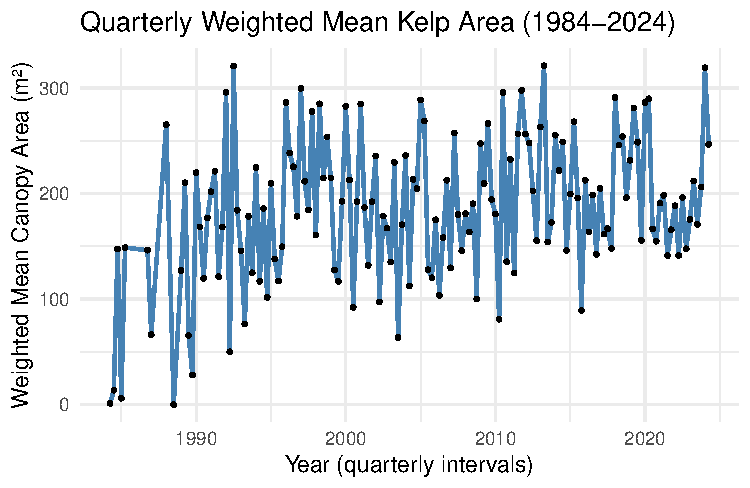
\includegraphics[width=0.6\linewidth,height=\textheight,keepaspectratio]{BCB744_Biostats_Prac_Exam_2025_files/figure-pdf/chunk6-1.pdf}
\end{center}

\begin{enumerate}
\def\labelenumi{\arabic{enumi}.}
\setcounter{enumi}{1}
\tightlist
\item
  Compute the weighted mean \texttt{area} at each unique
  (\texttt{longitude}, \texttt{latitude}) pixel across \texttt{time}.
  Then:
\end{enumerate}

\begin{itemize}
\tightlist
\item
  select a random sample of 100 pixels;
\item
  for each sampled pixel, extract the full time series of weighted mean
  area;
\item
  plot all 100 time series in a single panel (overlayed), using
  semi-transparent lines; and
\item
  label axes appropriately.
\end{itemize}

\textbf{Answer}

\textbf{\emph{Note to assessor:}} Again, if they produced the figure
exactly as below, this question can get full marks. Else, assess the
analysis workflow and assign marks in accordance with the portions of
the script that are correctly executed.

\begin{Shaded}
\begin{Highlighting}[]
\NormalTok{pixel\_means }\OtherTok{\textless{}{-}}\NormalTok{ long\_df }\SpecialCharTok{|\textgreater{}} 
  \FunctionTok{filter}\NormalTok{(}\SpecialCharTok{!}\FunctionTok{is.na}\NormalTok{(area), }\SpecialCharTok{!}\FunctionTok{is.na}\NormalTok{(passes), passes }\SpecialCharTok{\textgreater{}} \DecValTok{0}\NormalTok{) }\SpecialCharTok{|\textgreater{}} 
  \FunctionTok{group\_by}\NormalTok{(year, quarter, longitude, latitude) }\SpecialCharTok{|\textgreater{}} 
  \FunctionTok{summarise}\NormalTok{(}
    \AttributeTok{weighted\_area =} \FunctionTok{weighted.mean}\NormalTok{(area, }\AttributeTok{w =}\NormalTok{ passes, }\AttributeTok{na.rm =} \ConstantTok{TRUE}\NormalTok{),}
    \AttributeTok{.groups =} \StringTok{"drop"}
\NormalTok{  )}

\FunctionTok{summary}\NormalTok{(pixel\_means)}
\end{Highlighting}
\end{Shaded}

\begin{verbatim}
      year         quarter        longitude        latitude     
 Min.   :1984   Min.   :1.000   Min.   :15.08   Min.   :-34.83  
 1st Qu.:1997   1st Qu.:2.000   1st Qu.:18.33   1st Qu.:-34.67  
 Median :2006   Median :3.000   Median :18.84   Median :-34.36  
 Mean   :2006   Mean   :2.503   Mean   :18.64   Mean   :-33.62  
 3rd Qu.:2016   3rd Qu.:3.000   3rd Qu.:19.41   3rd Qu.:-33.95  
 Max.   :2024   Max.   :4.000   Max.   :19.97   Max.   :-26.48  
 weighted_area  
 Min.   :  0.0  
 1st Qu.:  0.0  
 Median :  0.0  
 Mean   :196.1  
 3rd Qu.:360.0  
 Max.   :900.0  
\end{verbatim}

\begin{Shaded}
\begin{Highlighting}[]
\CommentTok{\# Step 1: Calculate weighted mean per pixel over time}
\NormalTok{pixel\_means }\OtherTok{\textless{}{-}}\NormalTok{ long\_df }\SpecialCharTok{|\textgreater{}} 
  \FunctionTok{filter}\NormalTok{(}\SpecialCharTok{!}\FunctionTok{is.na}\NormalTok{(area), }\SpecialCharTok{!}\FunctionTok{is.na}\NormalTok{(passes), passes }\SpecialCharTok{\textgreater{}} \DecValTok{0}\NormalTok{) }\SpecialCharTok{|\textgreater{}} 
  \FunctionTok{group\_by}\NormalTok{(year, quarter, longitude, latitude) }\SpecialCharTok{|\textgreater{}} 
  \FunctionTok{summarise}\NormalTok{(}
    \AttributeTok{weighted\_area =} \FunctionTok{weighted.mean}\NormalTok{(area, }\AttributeTok{w =}\NormalTok{ passes, }\AttributeTok{na.rm =} \ConstantTok{TRUE}\NormalTok{),}
    \AttributeTok{.groups =} \StringTok{"drop"}
\NormalTok{  ) }\SpecialCharTok{|\textgreater{}} 
  \FunctionTok{mutate}\NormalTok{(}\AttributeTok{time\_index =}\NormalTok{ year }\SpecialCharTok{+}\NormalTok{ (quarter }\SpecialCharTok{{-}} \DecValTok{1}\NormalTok{) }\SpecialCharTok{/} \DecValTok{4}\NormalTok{)}

\CommentTok{\# Step 2: Identify 100 unique (lon, lat) pairs}
\FunctionTok{set.seed}\NormalTok{(}\DecValTok{42}\NormalTok{)}
\NormalTok{sample\_pixels }\OtherTok{\textless{}{-}}\NormalTok{ pixel\_means }\SpecialCharTok{|\textgreater{}} 
  \FunctionTok{distinct}\NormalTok{(longitude, latitude) }\SpecialCharTok{|\textgreater{}} 
  \FunctionTok{sample\_n}\NormalTok{(}\DecValTok{100}\NormalTok{)}

\CommentTok{\# Step 3: Filter time series for the sampled pixels}
\NormalTok{pixel\_timeseries\_sample }\OtherTok{\textless{}{-}}\NormalTok{ pixel\_means }\SpecialCharTok{|\textgreater{}} 
  \FunctionTok{inner\_join}\NormalTok{(sample\_pixels, }\AttributeTok{by =} \FunctionTok{c}\NormalTok{(}\StringTok{"longitude"}\NormalTok{, }\StringTok{"latitude"}\NormalTok{))}

\CommentTok{\# Step 4: Plot all 100 pixel time series}
\FunctionTok{ggplot}\NormalTok{(pixel\_timeseries\_sample,}
       \FunctionTok{aes}\NormalTok{(}\AttributeTok{x =}\NormalTok{ time\_index, }\AttributeTok{y =}\NormalTok{ weighted\_area,}
           \AttributeTok{group =} \FunctionTok{interaction}\NormalTok{(longitude, latitude))) }\SpecialCharTok{+}
  \FunctionTok{geom\_line}\NormalTok{(}\AttributeTok{alpha =} \FloatTok{0.3}\NormalTok{, }\AttributeTok{color =} \StringTok{"darkorange"}\NormalTok{) }\SpecialCharTok{+}
  \FunctionTok{labs}\NormalTok{(}
    \AttributeTok{title =} \StringTok{"Kelp Area Time Series for 100 Random Pixels"}\NormalTok{,}
    \AttributeTok{x =} \StringTok{"Year (quarterly intervals)"}\NormalTok{,}
    \AttributeTok{y =} \StringTok{"Weighted Mean Canopy Area (m²)"}
\NormalTok{  ) }\SpecialCharTok{+}
  \FunctionTok{theme\_minimal}\NormalTok{()}
\end{Highlighting}
\end{Shaded}

\begin{center}
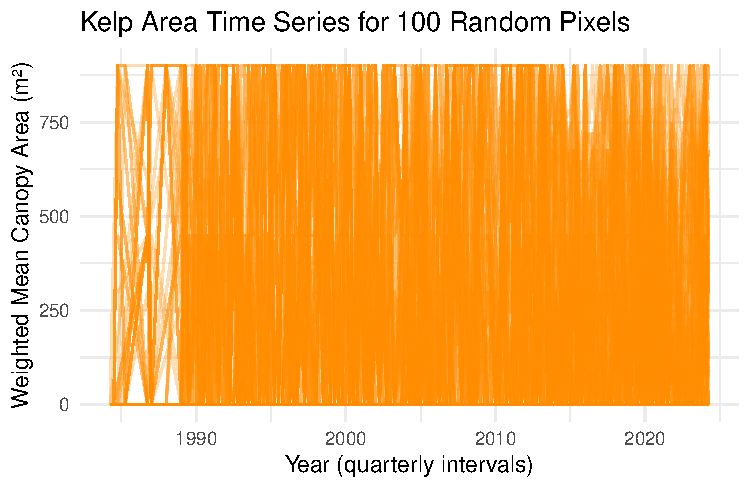
\includegraphics[width=0.6\linewidth,height=\textheight,keepaspectratio]{BCB744_Biostats_Prac_Exam_2025_files/figure-pdf/chunk7-1.pdf}
\end{center}

\begin{Shaded}
\begin{Highlighting}[]
\CommentTok{\# This figure is uninterpretable...}
\end{Highlighting}
\end{Shaded}

\subsubsection{2.2 Summary Statistics}\label{summary-statistics}

\begin{enumerate}
\def\labelenumi{\arabic{enumi}.}
\tightlist
\item
  Using the weighted data prepared for each \texttt{year} and
  \texttt{quarter} combination (prepared in 2.1.1), compute and report
  summary statistics for the levels of temporal aggregation:

  \begin{itemize}
  \tightlist
  \item
    by \texttt{year};
  \item
    by \texttt{quarter};
  \item
    by \texttt{year/quarter} combination;
  \end{itemize}
\end{enumerate}

\begin{itemize}
\tightlist
\item
  include: weighted mean, median, standard deviation, interquartile
  range, skewness, and kurtosis; and
\item
  comment on the appropriateness of each statistic for these data, and
  justify your choices in light of the data distribution.
\end{itemize}

\textbf{Answer}

\textbf{\emph{Note to assessor:}} Since this question can be objectively
assessed relative to the expectations (specific reporting of correct
summary stats per each level of aggregation as I have them below), marks
can simply be assigned based on the correct reporting of the summary
statistics.

\begin{Shaded}
\begin{Highlighting}[]
\FunctionTok{library}\NormalTok{(e1071)  }\CommentTok{\# for skewness and kurtosis}

\CommentTok{\# Yearly aggregation}
\NormalTok{year\_stats }\OtherTok{\textless{}{-}}\NormalTok{ quarter\_means }\SpecialCharTok{|\textgreater{}} 
  \FunctionTok{group\_by}\NormalTok{(year) }\SpecialCharTok{|\textgreater{}} 
  \FunctionTok{summarise}\NormalTok{(}
    \AttributeTok{mean =} \FunctionTok{mean}\NormalTok{(weighted\_area, }\AttributeTok{na.rm =} \ConstantTok{TRUE}\NormalTok{),}
    \AttributeTok{median =} \FunctionTok{median}\NormalTok{(weighted\_area, }\AttributeTok{na.rm =} \ConstantTok{TRUE}\NormalTok{),}
    \AttributeTok{sd =} \FunctionTok{sd}\NormalTok{(weighted\_area, }\AttributeTok{na.rm =} \ConstantTok{TRUE}\NormalTok{),}
    \AttributeTok{iqr =} \FunctionTok{IQR}\NormalTok{(weighted\_area, }\AttributeTok{na.rm =} \ConstantTok{TRUE}\NormalTok{),}
    \AttributeTok{skew =} \FunctionTok{skewness}\NormalTok{(weighted\_area, }\AttributeTok{na.rm =} \ConstantTok{TRUE}\NormalTok{),}
    \AttributeTok{kurt =} \FunctionTok{kurtosis}\NormalTok{(weighted\_area, }\AttributeTok{na.rm =} \ConstantTok{TRUE}\NormalTok{)}
\NormalTok{  )}
\NormalTok{year\_stats}
\end{Highlighting}
\end{Shaded}

\begin{verbatim}
# A tibble: 41 x 7
        year  mean median    sd   iqr     skew   kurt
   <int[1d]> <dbl>  <dbl> <dbl> <dbl>    <dbl>  <dbl>
 1      1984  54.1   13.6  81.2  73.2   0.375   -2.33
 2      1985  77.4   77.4 101.   71.4   0       -2.75
 3      1986 146.   146.   NA     0   NaN      NaN   
 4      1987  66.3   66.3  NA     0   NaN      NaN   
 5      1988 133.   133.  188.  133.    0       -2.75
 6      1989 108.    96.3  79.7  91.8   0.250   -2.04
 7      1990 171.   173.   41.1  31.5  -0.0806  -1.89
 8      1991 178.   185.   43.8  50.2  -0.272   -2.03
 9      1992 213.   240.  124.  152.   -0.329   -2.05
10      1993 131.   135.   42.8  41.1  -0.191   -1.95
# i 31 more rows
\end{verbatim}

\begin{Shaded}
\begin{Highlighting}[]
\CommentTok{\# Quarterly aggregation (across all years)}
\NormalTok{quarter\_stats }\OtherTok{\textless{}{-}}\NormalTok{ quarter\_means }\SpecialCharTok{|\textgreater{}} 
  \FunctionTok{group\_by}\NormalTok{(quarter) }\SpecialCharTok{|\textgreater{}} 
  \FunctionTok{summarise}\NormalTok{(}
    \AttributeTok{mean =} \FunctionTok{mean}\NormalTok{(weighted\_area, }\AttributeTok{na.rm =} \ConstantTok{TRUE}\NormalTok{),}
    \AttributeTok{median =} \FunctionTok{median}\NormalTok{(weighted\_area, }\AttributeTok{na.rm =} \ConstantTok{TRUE}\NormalTok{),}
    \AttributeTok{sd =} \FunctionTok{sd}\NormalTok{(weighted\_area, }\AttributeTok{na.rm =} \ConstantTok{TRUE}\NormalTok{),}
    \AttributeTok{iqr =} \FunctionTok{IQR}\NormalTok{(weighted\_area, }\AttributeTok{na.rm =} \ConstantTok{TRUE}\NormalTok{),}
    \AttributeTok{skew =} \FunctionTok{skewness}\NormalTok{(weighted\_area, }\AttributeTok{na.rm =} \ConstantTok{TRUE}\NormalTok{),}
    \AttributeTok{kurt =} \FunctionTok{kurtosis}\NormalTok{(weighted\_area, }\AttributeTok{na.rm =} \ConstantTok{TRUE}\NormalTok{)}
\NormalTok{  )}
\NormalTok{quarter\_stats}
\end{Highlighting}
\end{Shaded}

\begin{verbatim}
# A tibble: 4 x 7
  quarter  mean median    sd   iqr   skew    kurt
    <int> <dbl>  <dbl> <dbl> <dbl>  <dbl>   <dbl>
1       1  216.   220.  66.6  83.4 -0.898  0.922 
2       2  185.   204.  74.2 114.  -0.361 -0.598 
3       3  172.   179.  71.2  85.6 -0.326 -0.0222
4       4  166.   166.  49.7  46.2  0.177  1.32  
\end{verbatim}

\begin{Shaded}
\begin{Highlighting}[]
\CommentTok{\# Year{-}quarter combination (already in quarter\_means)}
\NormalTok{year\_quarter\_stats }\OtherTok{\textless{}{-}}\NormalTok{ quarter\_means }\SpecialCharTok{|\textgreater{}} 
  \FunctionTok{mutate}\NormalTok{(}\AttributeTok{year\_quarter =} \FunctionTok{paste0}\NormalTok{(year, }\StringTok{" Q"}\NormalTok{, quarter)) }\SpecialCharTok{|\textgreater{}} 
  \FunctionTok{summarise}\NormalTok{(}
    \AttributeTok{mean =} \FunctionTok{mean}\NormalTok{(weighted\_area, }\AttributeTok{na.rm =} \ConstantTok{TRUE}\NormalTok{),}
    \AttributeTok{median =} \FunctionTok{median}\NormalTok{(weighted\_area, }\AttributeTok{na.rm =} \ConstantTok{TRUE}\NormalTok{),}
    \AttributeTok{sd =} \FunctionTok{sd}\NormalTok{(weighted\_area, }\AttributeTok{na.rm =} \ConstantTok{TRUE}\NormalTok{),}
    \AttributeTok{iqr =} \FunctionTok{IQR}\NormalTok{(weighted\_area, }\AttributeTok{na.rm =} \ConstantTok{TRUE}\NormalTok{),}
    \AttributeTok{skew =} \FunctionTok{skewness}\NormalTok{(weighted\_area, }\AttributeTok{na.rm =} \ConstantTok{TRUE}\NormalTok{),}
    \AttributeTok{kurt =} \FunctionTok{kurtosis}\NormalTok{(weighted\_area, }\AttributeTok{na.rm =} \ConstantTok{TRUE}\NormalTok{)}
\NormalTok{  )}
\NormalTok{year\_quarter\_stats}
\end{Highlighting}
\end{Shaded}

\begin{verbatim}
# A tibble: 1 x 6
   mean median    sd   iqr   skew     kurt
  <dbl>  <dbl> <dbl> <dbl>  <dbl>    <dbl>
1  185.   186.  68.3  86.2 -0.323 -0.00284
\end{verbatim}

\begin{enumerate}
\def\labelenumi{\arabic{enumi}.}
\setcounter{enumi}{1}
\tightlist
\item
  Create visualisations (e.g.~boxplots, violin plots, histograms) to
  support your interpretations.
\end{enumerate}

\textbf{Answer}

\textbf{\emph{Note to assessor:}} These or similar figures are required,
showing the seasonal effects, the annual effect, a histogram of the
frequency of the weighted areas, and something similar to the density
distribution (or a frequency histogram) that shows distribution within a
quarter. I'd also accept variations of these plots, as long as they
speak to the nature of the data being assessed. They need to capture the
feature of the summary statistics that I have above.

\begin{Shaded}
\begin{Highlighting}[]
\CommentTok{\# Boxplot by quarter}
\FunctionTok{ggplot}\NormalTok{(quarter\_means, }\FunctionTok{aes}\NormalTok{(}\AttributeTok{x =} \FunctionTok{factor}\NormalTok{(quarter), }\AttributeTok{y =}\NormalTok{ weighted\_area)) }\SpecialCharTok{+}
  \FunctionTok{geom\_boxplot}\NormalTok{(}\AttributeTok{fill =} \StringTok{"lightblue"}\NormalTok{) }\SpecialCharTok{+}
  \FunctionTok{labs}\NormalTok{(}\AttributeTok{title =} \StringTok{"Kelp Canopy Area by Quarter"}\NormalTok{,}
       \AttributeTok{x =} \StringTok{"Quarter"}\NormalTok{, }\AttributeTok{y =} \StringTok{"Weighted Area"}\NormalTok{) }\SpecialCharTok{+}
  \FunctionTok{theme\_minimal}\NormalTok{()}
\end{Highlighting}
\end{Shaded}

\begin{center}
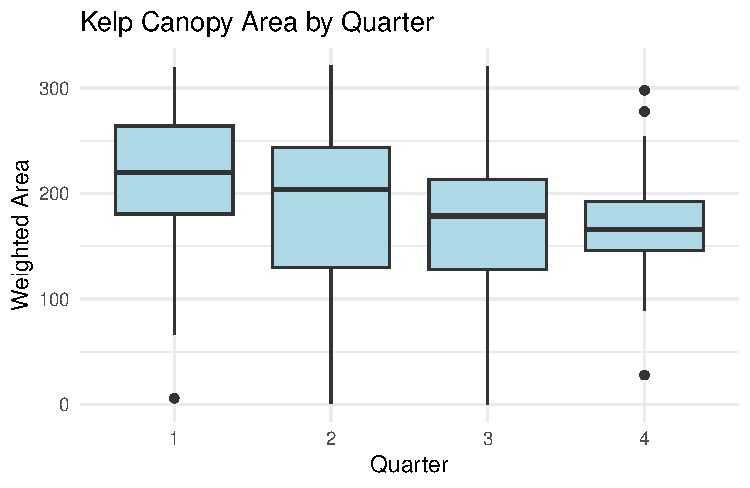
\includegraphics[width=0.6\linewidth,height=\textheight,keepaspectratio]{BCB744_Biostats_Prac_Exam_2025_files/figure-pdf/chunk9-1.pdf}
\end{center}

\begin{Shaded}
\begin{Highlighting}[]
\CommentTok{\# Boxplot by year}
\FunctionTok{ggplot}\NormalTok{(quarter\_means, }\FunctionTok{aes}\NormalTok{(}\AttributeTok{x =} \FunctionTok{factor}\NormalTok{(year), }\AttributeTok{y =}\NormalTok{ weighted\_area)) }\SpecialCharTok{+}
  \FunctionTok{geom\_boxplot}\NormalTok{(}\AttributeTok{fill =} \StringTok{"lightgreen"}\NormalTok{) }\SpecialCharTok{+}
  \FunctionTok{labs}\NormalTok{(}\AttributeTok{title =} \StringTok{"Kelp Canopy Area by Year"}\NormalTok{,}
       \AttributeTok{x =} \StringTok{"Year"}\NormalTok{, }\AttributeTok{y =} \StringTok{"Weighted Area"}\NormalTok{) }\SpecialCharTok{+}
  \FunctionTok{theme\_minimal}\NormalTok{() }\SpecialCharTok{+}
  \FunctionTok{theme}\NormalTok{(}\AttributeTok{axis.text.x =} \FunctionTok{element\_text}\NormalTok{(}\AttributeTok{angle =} \DecValTok{90}\NormalTok{, }\AttributeTok{hjust =} \DecValTok{1}\NormalTok{))}
\end{Highlighting}
\end{Shaded}

\begin{center}
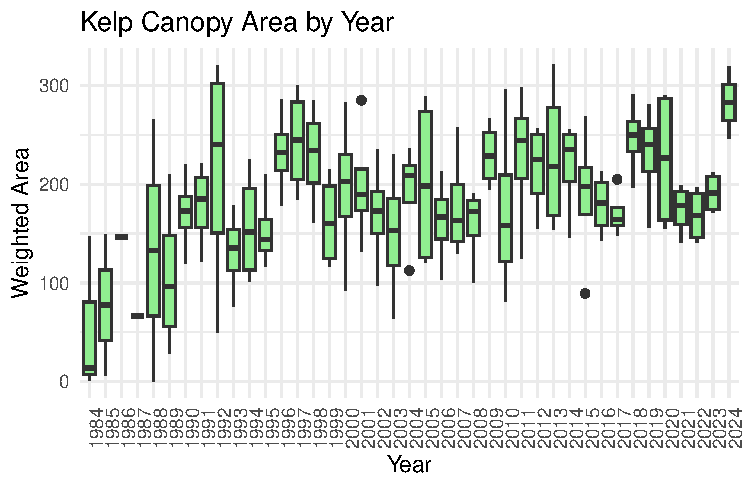
\includegraphics[width=12cm,height=\textheight,keepaspectratio]{BCB744_Biostats_Prac_Exam_2025_files/figure-pdf/chunk9-2.pdf}
\end{center}

\begin{Shaded}
\begin{Highlighting}[]
\CommentTok{\# Histogram of all weighted areas}
\FunctionTok{ggplot}\NormalTok{(quarter\_means, }\FunctionTok{aes}\NormalTok{(}\AttributeTok{x =}\NormalTok{ weighted\_area)) }\SpecialCharTok{+}
  \FunctionTok{geom\_histogram}\NormalTok{(}\AttributeTok{bins =} \DecValTok{30}\NormalTok{, }\AttributeTok{fill =} \StringTok{"tan"}\NormalTok{, }\AttributeTok{color =} \StringTok{"black"}\NormalTok{) }\SpecialCharTok{+}
  \FunctionTok{labs}\NormalTok{(}\AttributeTok{title =} \StringTok{"Histogram of Weighted Kelp Area"}\NormalTok{,}
       \AttributeTok{x =} \StringTok{"Weighted Area"}\NormalTok{, }\AttributeTok{y =} \StringTok{"Frequency"}\NormalTok{) }\SpecialCharTok{+}
  \FunctionTok{theme\_minimal}\NormalTok{()}
\end{Highlighting}
\end{Shaded}

\begin{center}
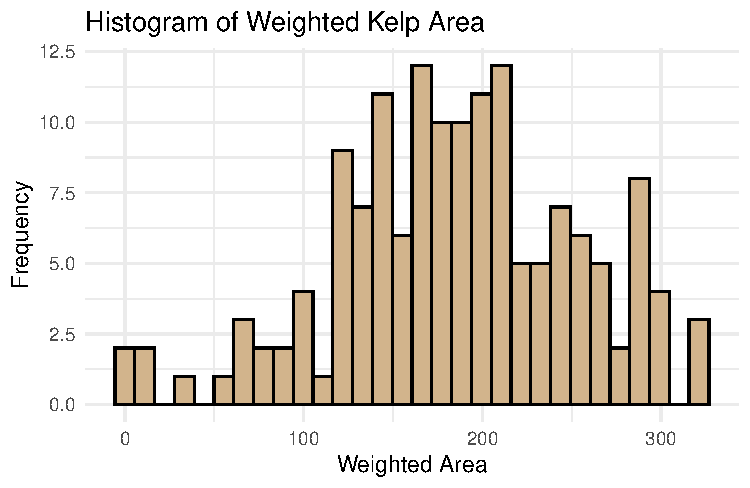
\includegraphics[width=0.6\linewidth,height=\textheight,keepaspectratio]{BCB744_Biostats_Prac_Exam_2025_files/figure-pdf/chunk9-3.pdf}
\end{center}

\begin{Shaded}
\begin{Highlighting}[]
\CommentTok{\# Density plot by quarter}
\FunctionTok{ggplot}\NormalTok{(quarter\_means, }\FunctionTok{aes}\NormalTok{(}\AttributeTok{x =}\NormalTok{ weighted\_area, }\AttributeTok{color =} \FunctionTok{factor}\NormalTok{(quarter))) }\SpecialCharTok{+}
  \FunctionTok{geom\_density}\NormalTok{() }\SpecialCharTok{+}
  \FunctionTok{labs}\NormalTok{(}\AttributeTok{title =} \StringTok{"Density of Weighted Area by Quarter"}\NormalTok{,}
       \AttributeTok{x =} \StringTok{"Weighted Area"}\NormalTok{, }\AttributeTok{color =} \StringTok{"Quarter"}\NormalTok{) }\SpecialCharTok{+}
  \FunctionTok{theme\_minimal}\NormalTok{()}
\end{Highlighting}
\end{Shaded}

\begin{center}
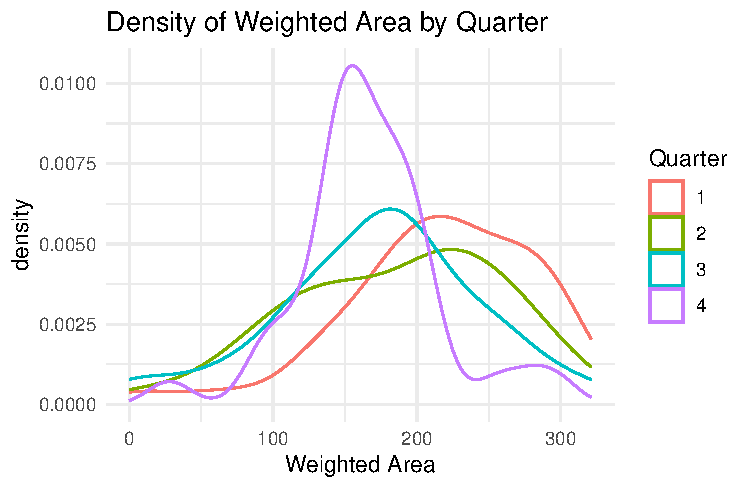
\includegraphics[width=12cm,height=\textheight,keepaspectratio]{BCB744_Biostats_Prac_Exam_2025_files/figure-pdf/chunk9-4.pdf}
\end{center}

\begin{enumerate}
\def\labelenumi{\arabic{enumi}.}
\setcounter{enumi}{2}
\tightlist
\item
  Based on these, discuss any discernible temporal trends (e.g.~decadal
  increases/decreases) and seasonal patterns (quarterly effects).
\end{enumerate}

\textbf{Answer}

\textbf{\emph{Note to assessor:}} Some variation of this:

Temporal variation in kelp canopy area, as observed in the quarterly
weighted means from 1984 to 2024, exhibits a broadly increasing trend
until the early-2000s, followed by more irregular fluctuations at a
higher weighted canopy area than at the start of the time series. The
yearly summary statistics confirm this, and show rising means and
medians through the late 1990s into the early 2000s, peaking during the
2010s. Although values for some early years (e.g., 1986, 1987) suffer
from missing data (e.g., NA for SD and skewness), the central decades
present coherent patterns.

The skewness values tend to hover close to zero, with mild left-skew in
later years, suggesting distributions that are not heavily distorted but
do include more frequent lower outliers in certain quarters. The
kurtosis estimates, consistently below 0 across many years, indicate
relatively flat distributions with light tails, again pointing to the
presence of moderate, widespread values and a paucity of extreme
outliers in the tails.

The quarterly summaries reveal a seasonal signal: Q1 (January--March) is
associated with the highest mean kelp area (216 km²), while Q4
(October--December) shows the lowest (166 km²). This likely reflects
seasonal growth dynamics, perhaps linked to photoperiod, wave exposure,
or nutrient regimes (factors known to modulate canopy) forming
macroalgae. The density plot by quarter reinforces this picture: Q1's
density curve is skewed leftward, indicative of a modal concentration
around high values, whereas Q4 shows more compact distributions with
lower peaks.

The boxplots by year reinforce this temporal variation. Inter-annual
variation is relatively low during some periods (e.g., 1990s) but
expands considerably in the 2010s and 2020s, suggesting a greater degree
of spatial heterogeneity or more frequent episodes of extreme coverage.
Notably, the increase in spread does not always correspond with a
decline in median or mean area, implying that while certain coastal
sectors may experience loss, others persist or expand.

The histogram of weighted area suggests a right-skewed global
distribution when pooled over time, driven by many instances of low or
zero canopy and fewer but notable high-coverage events.

So, these patterns suggest:

\begin{itemize}
\tightlist
\item
  A long-term trend toward increased kelp canopy extent over the study
  period, potentially stabilising or fragmenting in recent years;
\item
  Clear intra-annual (seasonal) variation, with Q1 consistently
  supporting greater canopy development than later quarters;
\item
  Increasing variability over time, which might reflect changing climate
  regimes, hydrodynamic forcing, or anthropogenic disturbance gradients.
\end{itemize}

These findings provide a strong descriptive foundation for the
inferential modelling that follows.

\subsubsection{2.3 Observation Density
Map}\label{observation-density-map}

Create a map plotting each observed pixel location (defined by
\texttt{longitude} × \texttt{latitude}):

\begin{itemize}
\tightlist
\item
  colour each pixel by the total number of valid observations (i.e.,
  non-NA values of \texttt{area}) across all \texttt{time} points;
\item
  overlay the 58 coastal sections as reference points or lines, numbered
  from west (1) to east (58); and
\item
  use an appropriate geographic projection and include a legend.
\end{itemize}

\textbf{Answer}

\textbf{\emph{Note to assessor:}} I'm not concerned too much about
having a coastline as the data clearly show the coastal profile, but, of
course, having the coastline as well is great too (maybe worth a mark or
three extra). I'd also be okay if the figure focuses only on sections
1-22 where kelp is present. Again, this is a fairly objective question,
so marks can be assigned based on the correct figure (full marks for all
the labels, etc., correctly applied as per standards of scientific
publications).

\begin{Shaded}
\begin{Highlighting}[]
\FunctionTok{library}\NormalTok{(ggrepel)  }\CommentTok{\# for labelling points}
\FunctionTok{library}\NormalTok{(viridis)  }\CommentTok{\# for color scale}

\CommentTok{\# Load the long\_df and coastal sections}
\CommentTok{\# Assume long\_df has already been created from earlier tasks}
\CommentTok{\# Load the 58 sections file (replace with actual path if needed)}
\NormalTok{sections\_df }\OtherTok{\textless{}{-}} \FunctionTok{read.csv}\NormalTok{(}\StringTok{"../data/Kelpwatch/58\_sections.csv"}\NormalTok{)}

\CommentTok{\# 1. Count valid observations per pixel}
\NormalTok{obs\_counts }\OtherTok{\textless{}{-}}\NormalTok{ long\_df }\SpecialCharTok{|\textgreater{}} 
  \FunctionTok{filter}\NormalTok{(}\SpecialCharTok{!}\FunctionTok{is.na}\NormalTok{(area)) }\SpecialCharTok{|\textgreater{}} 
  \FunctionTok{group\_by}\NormalTok{(longitude, latitude) }\SpecialCharTok{|\textgreater{}} 
  \FunctionTok{summarise}\NormalTok{(}
    \AttributeTok{n\_obs =} \FunctionTok{n}\NormalTok{(),}
    \AttributeTok{.groups =} \StringTok{"drop"}
\NormalTok{  )}

\CommentTok{\# 2. Prepare coastal sections data}
\NormalTok{sections }\OtherTok{\textless{}{-}}\NormalTok{ sections\_df }\SpecialCharTok{|\textgreater{}} 
  \FunctionTok{mutate}\NormalTok{(}\AttributeTok{section\_id =} \FunctionTok{row\_number}\NormalTok{())}

\CommentTok{\# 3. Plot}
\FunctionTok{ggplot}\NormalTok{() }\SpecialCharTok{+}
  \FunctionTok{geom\_point}\NormalTok{(}
    \AttributeTok{data =}\NormalTok{ obs\_counts, }\AttributeTok{shape =} \DecValTok{4}\NormalTok{,}
    \FunctionTok{aes}\NormalTok{(}\AttributeTok{x =}\NormalTok{ longitude, }\AttributeTok{y =}\NormalTok{ latitude, }\AttributeTok{colour =}\NormalTok{ n\_obs)}
\NormalTok{    ) }\SpecialCharTok{+}
  \FunctionTok{scale\_colour\_viridis}\NormalTok{(}\AttributeTok{name =} \StringTok{"Valid}\SpecialCharTok{\textbackslash{}n}\StringTok{Obs."}\NormalTok{, }\AttributeTok{option =} \StringTok{"plasma"}\NormalTok{) }\SpecialCharTok{+}
  \FunctionTok{geom\_point}\NormalTok{(}
    \AttributeTok{data =}\NormalTok{ sections,}
    \AttributeTok{color =} \StringTok{"black"}\NormalTok{, }\AttributeTok{size =} \FloatTok{1.1}\NormalTok{, }\AttributeTok{shape =} \DecValTok{1}\NormalTok{,}
    \FunctionTok{aes}\NormalTok{(}\AttributeTok{x =}\NormalTok{ Longitude, }\AttributeTok{y =}\NormalTok{ Latitude)}
\NormalTok{    ) }\SpecialCharTok{+}
  \FunctionTok{geom\_text\_repel}\NormalTok{(}
    \AttributeTok{data =}\NormalTok{ sections,}
    \AttributeTok{size =} \DecValTok{2}\NormalTok{,}
    \AttributeTok{color =} \StringTok{"black"}\NormalTok{,}
    \AttributeTok{max.overlaps =} \DecValTok{58}\NormalTok{,}
    \FunctionTok{aes}\NormalTok{(}\AttributeTok{x =}\NormalTok{ Longitude, }\AttributeTok{y =}\NormalTok{ Latitude, }\AttributeTok{label =}\NormalTok{ section\_id)}
\NormalTok{  ) }\SpecialCharTok{+}
  \FunctionTok{coord\_fixed}\NormalTok{(}\FloatTok{1.3}\NormalTok{) }\SpecialCharTok{+}
  \FunctionTok{labs}\NormalTok{(}
    \AttributeTok{title =} \StringTok{"Observation Density Map"}\NormalTok{,}
    \AttributeTok{subtitle =} \StringTok{"Total no. valid kelp area obs. per pixel (1984–2024)"}\NormalTok{,}
    \AttributeTok{x =} \StringTok{"Longitude"}\NormalTok{,}
    \AttributeTok{y =} \StringTok{"Latitude"}
\NormalTok{  ) }\SpecialCharTok{+}
  \FunctionTok{theme\_minimal}\NormalTok{()}
\end{Highlighting}
\end{Shaded}

\begin{center}
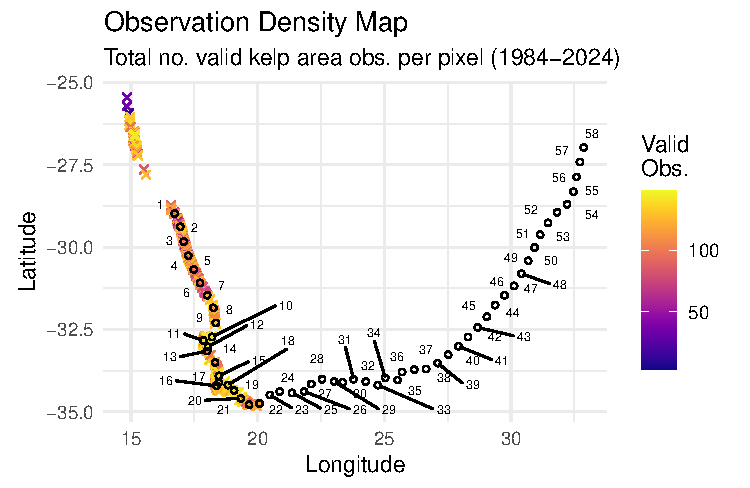
\includegraphics[width=0.6\linewidth,height=\textheight,keepaspectratio]{BCB744_Biostats_Prac_Exam_2025_files/figure-pdf/chunk10-1.pdf}
\end{center}

\subsection{Task 3: Inferential Statistics (Part
1)}\label{task-3-inferential-statistics-part-1}

\begin{itemize}
\tightlist
\item
  \textbf{{[}Task Weight: 20\%{]}}
\item
  \textbf{{[}Components (1), (2), (3), and (4) each marked on a 0--100
  scale, then scaled to equal proportions of the Task Weight of 20\%{]}}
\end{itemize}

You are now asked to formally test whether the weighted mean kelp canopy
area has changed over time, and whether it shows evidence of seasonal
variation.

You should:

\begin{enumerate}
\def\labelenumi{\arabic{enumi}.}
\tightlist
\item
  Formulate and clearly state the null and alternative hypotheses for
  each of the following:

  \begin{itemize}
  \tightlist
  \item
    a temporal effect (i.e., whether kelp canopy area has changed across
    the study period); and
  \item
    a seasonal effect (i.e., whether kelp canopy area differs between
    quarters).
  \end{itemize}
\end{enumerate}

\textbf{Answer}

\textbf{\emph{Note to assessor:}} The null and alternative hypotheses
can be clearly and strictly stated as I have them. This provides strong
and an unambiguous basis for the inferential tests that follow, and
marks should be assigned accordingly (questions 1-4).

Temporal effect (across years):

\begin{itemize}
\tightlist
\item
  H0: There is no effect of year on kelp canopy area.
\item
  H1: There is a significant effect of year on kelp canopy area.
\end{itemize}

Seasonal effect (across quarters):

\begin{itemize}
\tightlist
\item
  H0: There is no effect of quarter on kelp canopy area.
\item
  H1: There is a significant effect of quarter on kelp canopy area.
\end{itemize}

\begin{enumerate}
\def\labelenumi{\arabic{enumi}.}
\setcounter{enumi}{1}
\tightlist
\item
  Choose and implement a statistical model appropriate to this task.
\end{enumerate}

You may also consider:

\begin{itemize}
\tightlist
\item
  whether to model individual observations or to aggregate the data
  across spatial pixels; and
\item
  how to treat missing or zero-valued observations.
\end{itemize}

The model you choose should reflect your understanding of the data
structure and the nature of the questions being asked.

\textbf{Answer}

\textbf{\emph{Note to assessor:}} Given the relatively small number of
observations (n = 164 quarters over 41 years), and the fact that these
are weighted mean values (not raw spatially disaggregated pixels), a
linear model is appropriate. We'll use \texttt{lm()} here with both year
and quarter as additive predictors, but I'll also accept a linear model
to test for the \texttt{year} effect and an ANOVA to test the
\texttt{quarter} effect. However, I prefer the \texttt{lm()} as it is
more inclusive, comprehensive, and efficient. I did not specifically ask
for an interaction effect, so no extra marks for assessing the
interaction term.

\begin{Shaded}
\begin{Highlighting}[]
\CommentTok{\# Ensure correct types}
\NormalTok{quarter\_means }\OtherTok{\textless{}{-}}\NormalTok{ quarter\_means }\SpecialCharTok{|\textgreater{}} 
  \FunctionTok{mutate}\NormalTok{(}
    \AttributeTok{year =} \FunctionTok{as.integer}\NormalTok{(year),}
    \AttributeTok{quarter =} \FunctionTok{factor}\NormalTok{(quarter) }\CommentTok{\# categorical, not numeric}
\NormalTok{  )}

\CommentTok{\# Fit additive model: weighted area \textasciitilde{} year + quarter}
\NormalTok{lm\_additive }\OtherTok{\textless{}{-}} \FunctionTok{lm}\NormalTok{(weighted\_area }\SpecialCharTok{\textasciitilde{}}\NormalTok{ year }\SpecialCharTok{+}\NormalTok{ quarter, }\AttributeTok{data =}\NormalTok{ quarter\_means)}

\CommentTok{\# Summary of the model}
\FunctionTok{summary}\NormalTok{(lm\_additive)}
\end{Highlighting}
\end{Shaded}

\begin{verbatim}

Call:
lm(formula = weighted_area ~ year + quarter, data = quarter_means)

Residuals:
     Min       1Q   Median       3Q      Max 
-170.137  -42.569    4.579   40.684  174.330 

Coefficients:
              Estimate Std. Error t value Pr(>|t|)    
(Intercept) -3751.4614   921.5608  -4.071 7.65e-05 ***
year            1.9786     0.4596   4.305 3.05e-05 ***
quarter2      -31.0695    14.2591  -2.179 0.030941 *  
quarter3      -43.5227    14.3554  -3.032 0.002877 ** 
quarter4      -49.3584    14.3555  -3.438 0.000763 ***
---
Signif. codes:  0 '***' 0.001 '**' 0.01 '*' 0.05 '.' 0.1 ' ' 1

Residual standard error: 62.55 on 146 degrees of freedom
Multiple R-squared:  0.1838,    Adjusted R-squared:  0.1614 
F-statistic: 8.219 on 4 and 146 DF,  p-value: 5.25e-06
\end{verbatim}

\begin{Shaded}
\begin{Highlighting}[]
\CommentTok{\# I\textquotesingle{}d also accept simply two models that only look at year and season}
\CommentTok{\# as the main effects}
\end{Highlighting}
\end{Shaded}

\begin{enumerate}
\def\labelenumi{\arabic{enumi}.}
\setcounter{enumi}{2}
\tightlist
\item
  Justify your modelling approach, including:

  \begin{itemize}
  \tightlist
  \item
    why you chose that particular method (rather than alternatives);
  \item
    the assumptions involved; and
  \item
    how those assumptions might be violated in this dataset.
  \end{itemize}
\end{enumerate}

\textbf{Answer}

\textbf{\emph{Note to assessor:}} A linear model was selected to test
for additive effects of time (\texttt{year}, numeric) and seasonality
(\texttt{quarter}, categorical) on the weighted mean kelp canopy area.
This is justified by the structure of the quarter\_means dataset, which
is already aggregated by time and does not include repeated spatial
measurements that would justify a hierarchical or mixed model. The model
assumes independence of residuals, homoscedasticity, and approximate
normality of errors---conditions that are examined below.

A similar justification would be needed should the choice have been a
\texttt{lm()} for \texttt{year} and an \texttt{aov()} for
\texttt{quarter}.

It is plausible the the normality or heteroscedasity assumptions are
violated as a result of the slightly right-skewed data seen in an
earlier analysis. We will test these in the assumption tests which
follow.

\begin{enumerate}
\def\labelenumi{\arabic{enumi}.}
\setcounter{enumi}{3}
\tightlist
\item
  Present and interpret your results as you would in a scientific paper.
\end{enumerate}

\textbf{Answer}

\textbf{\emph{Note to assessor:}} The diagnostics might not be part of
the Results, but it should be reported somewhere to convince the
examiner that these were checked. It needs to be mentioned in the
Results (below) what the findings where to justify the test you
ultimately selected.

\begin{Shaded}
\begin{Highlighting}[]
\CommentTok{\# Default diagnostic plots}
\CommentTok{\# Set up compact margins and multi{-}panel layout}
\FunctionTok{par}\NormalTok{(}
  \AttributeTok{mfrow =} \FunctionTok{c}\NormalTok{(}\DecValTok{2}\NormalTok{, }\DecValTok{2}\NormalTok{),     }\CommentTok{\# 2 rows, 2 columns}
  \AttributeTok{mar =} \FunctionTok{c}\NormalTok{(}\DecValTok{4}\NormalTok{, }\DecValTok{4}\NormalTok{, }\DecValTok{2}\NormalTok{, }\DecValTok{1}\NormalTok{), }\CommentTok{\# inner margins: bottom, left, top, right}
  \AttributeTok{oma =} \FunctionTok{c}\NormalTok{(}\DecValTok{1}\NormalTok{, }\DecValTok{1}\NormalTok{, }\DecValTok{1}\NormalTok{, }\DecValTok{1}\NormalTok{)  }\CommentTok{\# outer margins}
\NormalTok{)}

\CommentTok{\# Plot standard lm diagnostics}
\FunctionTok{plot}\NormalTok{(lm\_additive)}
\end{Highlighting}
\end{Shaded}

\begin{center}
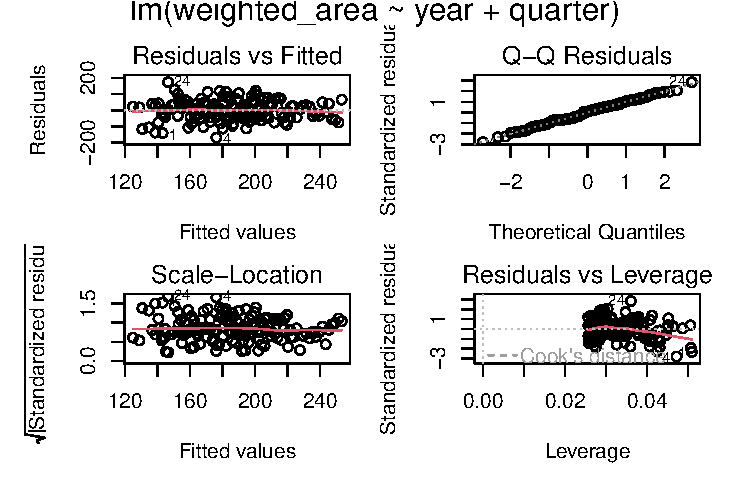
\includegraphics[width=0.6\linewidth,height=\textheight,keepaspectratio]{BCB744_Biostats_Prac_Exam_2025_files/figure-pdf/chunk12-1.pdf}
\end{center}

\begin{Shaded}
\begin{Highlighting}[]
\CommentTok{\# Reset to default layout afterwards}
\FunctionTok{par}\NormalTok{(}\AttributeTok{mfrow =} \FunctionTok{c}\NormalTok{(}\DecValTok{1}\NormalTok{, }\DecValTok{1}\NormalTok{))}
\end{Highlighting}
\end{Shaded}

These two figure will need to be reported with the Results, and
explained:

\begin{Shaded}
\begin{Highlighting}[]
\FunctionTok{anova}\NormalTok{(lm\_additive)}
\end{Highlighting}
\end{Shaded}

\begin{verbatim}
Analysis of Variance Table

Response: weighted_area
           Df Sum Sq Mean Sq F value    Pr(>F)    
year        1  72915   72915 18.6353 2.905e-05 ***
quarter     3  55724   18575  4.7472  0.003446 ** 
Residuals 146 571260    3913                      
---
Signif. codes:  0 '***' 0.001 '**' 0.01 '*' 0.05 '.' 0.1 ' ' 1
\end{verbatim}

\begin{Shaded}
\begin{Highlighting}[]
\CommentTok{\# Effect of year}
\FunctionTok{ggplot}\NormalTok{(quarter\_means, }\FunctionTok{aes}\NormalTok{(}\AttributeTok{x =}\NormalTok{ year, }\AttributeTok{y =}\NormalTok{ weighted\_area)) }\SpecialCharTok{+}
  \FunctionTok{geom\_point}\NormalTok{(}\AttributeTok{alpha =} \FloatTok{0.6}\NormalTok{) }\SpecialCharTok{+}
  \FunctionTok{geom\_smooth}\NormalTok{(}\AttributeTok{method =} \StringTok{"lm"}\NormalTok{, }\AttributeTok{se =} \ConstantTok{TRUE}\NormalTok{, }\AttributeTok{color =} \StringTok{"blue"}\NormalTok{) }\SpecialCharTok{+}
  \FunctionTok{labs}\NormalTok{(}\AttributeTok{title =} \StringTok{"Temporal Trend in Weighted Kelp Area"}\NormalTok{, }\AttributeTok{x =} \StringTok{"Year"}\NormalTok{, }\AttributeTok{y =} \StringTok{"Weighted Area"}\NormalTok{) }\SpecialCharTok{+}
  \FunctionTok{theme\_minimal}\NormalTok{()}
\end{Highlighting}
\end{Shaded}

\begin{center}
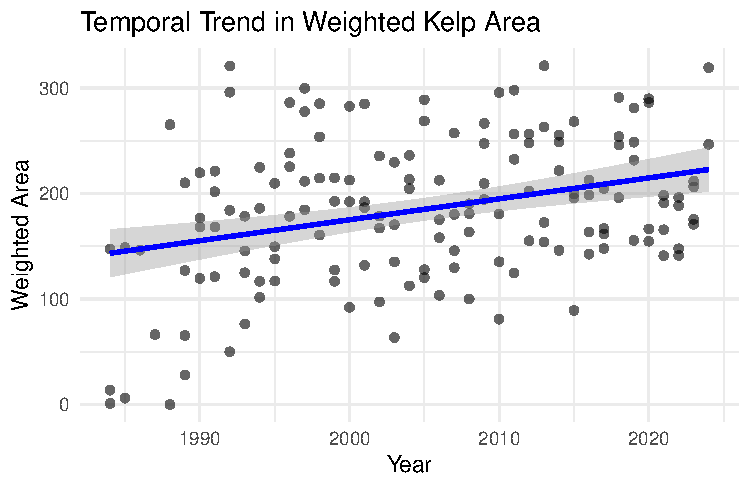
\includegraphics[width=0.6\linewidth,height=\textheight,keepaspectratio]{BCB744_Biostats_Prac_Exam_2025_files/figure-pdf/chunk13-1.pdf}
\end{center}

\begin{Shaded}
\begin{Highlighting}[]
\CommentTok{\# Effect of quarter}
\FunctionTok{ggplot}\NormalTok{(quarter\_means, }\FunctionTok{aes}\NormalTok{(}\AttributeTok{x =}\NormalTok{ quarter, }\AttributeTok{y =}\NormalTok{ weighted\_area)) }\SpecialCharTok{+}
  \FunctionTok{geom\_boxplot}\NormalTok{(}\AttributeTok{fill =} \StringTok{"lightgreen"}\NormalTok{) }\SpecialCharTok{+}
  \FunctionTok{labs}\NormalTok{(}\AttributeTok{title =} \StringTok{"Seasonal Variation in Weighted Kelp Area"}\NormalTok{, }\AttributeTok{x =} \StringTok{"Quarter"}\NormalTok{, }\AttributeTok{y =} \StringTok{"Weighted Area"}\NormalTok{) }\SpecialCharTok{+}
  \FunctionTok{theme\_minimal}\NormalTok{()}
\end{Highlighting}
\end{Shaded}

\begin{center}
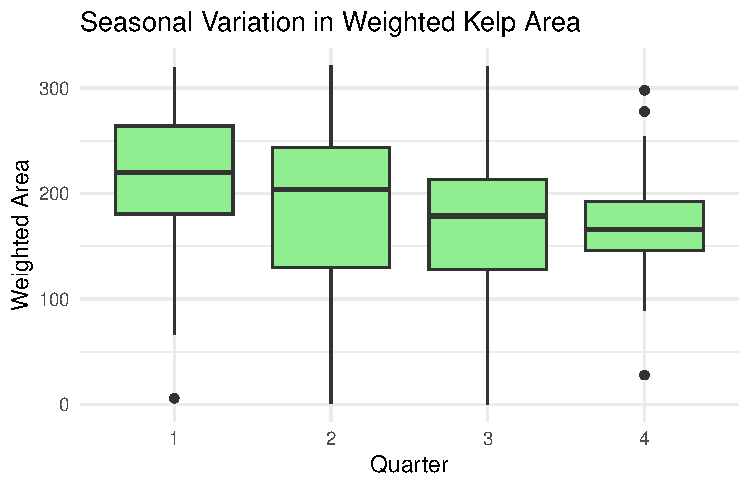
\includegraphics[width=12cm,height=\textheight,keepaspectratio]{BCB744_Biostats_Prac_Exam_2025_files/figure-pdf/chunk13-2.pdf}
\end{center}

\textbf{\emph{Results}} The linear model examining the additive effects
of year (numeric) and quarter (categorical) on quarterly weighted mean
kelp canopy area reveals two prominent patterns: a clear temporal trend
and a seasonal modulation of kelp cover (Figure x).

Regarding the temporal trend, the coefficient for year is positive and
statistically significant (\emph{β} = 1.98, \emph{p} \textless{} 0.001),
indicating a gradual increase in kelp canopy area over the 41-year
period. On average, the weighted canopy area increased by approximately
2 m² per year. This suggests a persistent long-term expansion of kelp
cover.

All three quarter indicators (Q2--Q4, with Q1 as reference) are
significantly negative, confirming that Q1 supports the highest canopy
cover (Figure y). The estimated differences range from −31 m² (Q2) to
−49 m² (Q4), all statistically significant at \emph{p} \textless{} 0.05.
This seasonal signal aligns with ecological expectations regarding
seasonal effects.

The model explains approximately 18\% of the total variance (R² = 0.18),
which, while slight, is reasonable for ecological time series aggregated
at the quarterly scale. Residual plots suggest approximate normality,
with slight heteroscedasticity at the extremes. The Q--Q plot exhibits
minor departures in the tails, but no worrying outliers or leverage
points compromise the fit. These diagnostics support the model's
suitability for inference, though future work might benefit from a more
flexible framework (e.g., GAMs) to account for potential nonlinearities.

These findings point to a persistent long-term increase in kelp canopy
cover along the South African coast, potentially reflecting broader
shifts in oceanographic or climatic regimes, such as changes in
upwelling intensity, nutrient flux, or wave climate. The consistent
seasonal signature, with maximal cover in Q1, supports the hypothesis of
photoperiod- or temperature-driven phenology. Notably, the lower cover
in Q4 might coincide with stormier periods or post-reproductive
senescence. Taken together, the temporal and seasonal dynamics provide a
robust baseline for assessing spatial heterogeneity and long-term
ecological change in subsequent tasks.

\subsection{Task 4: Assigning Kelp Observations to Coastal
Sections}\label{task-4-assigning-kelp-observations-to-coastal-sections}

\begin{itemize}
\tightlist
\item
  \textbf{{[}Task Weight: 20\%{]}}
\item
  \textbf{{[}Tasks 4.1 and 4.2 each marked on a 0--100 scale, then
  scaled in the proportion 0.7 and 0.3 of the Task Weight of 20\%{]}}
\end{itemize}

Using the data prepared above, your task now is to spatially classify
each kelp canopy observation by assigning it to two types of geographic
units.

\subsubsection{4.1 Assignment to Coastal
Sections}\label{assignment-to-coastal-sections}

You are provided with a table of 58 coastal sections, each defined by a
single geographic coordinate (\texttt{Latitude} and \texttt{Longitude}).
These points mark successive \textasciitilde50 km intervals along the
South African coastline, numbered from west (1) to east (58).

Assign each kelp canopy observation to the nearest coastal section based
on geographic proximity:

\begin{itemize}
\tightlist
\item
  use a geodesic (great-circle) distance metric to compute proximity
  between kelp sampling points and section coordinates (assume all
  coordinates are in WGS84);
\item
  add a new column to your kelp dataset called \texttt{section\_id},
  indicating the row number (1--58) of the nearest section; and
\item
  you may use any R packages or methods you like, but your code should
  be efficient and well-commented.
\end{itemize}

\textbf{Answer}

\textbf{\emph{Note to assessor:}} Check for objective evidence that a
dataframe has been created and that it has the correct columns, i.e.,
\texttt{section\_id} or \texttt{section}, \texttt{longitude},
\texttt{latitude}, \texttt{year}, \texttt{quarter}, and \texttt{area} or
\texttt{weighted\_area}. Calculations must show evidence of using the
Haversine distance metric.

I use only the relevant sections:

\begin{Shaded}
\begin{Highlighting}[]
\NormalTok{sections\_df }\OtherTok{\textless{}{-}}\NormalTok{ sections\_df }\SpecialCharTok{|\textgreater{}}
  \FunctionTok{slice}\NormalTok{(}\DecValTok{1}\SpecialCharTok{:}\DecValTok{22}\NormalTok{) }\CommentTok{\# no Ecklonia further east of section 22}
\end{Highlighting}
\end{Shaded}

Prepare a script for sectioning the kelp data:

\begin{Shaded}
\begin{Highlighting}[]
\NormalTok{processed\_file\_path }\OtherTok{\textless{}{-}} \StringTok{"../data/Kelpwatch/pixel\_means.RData"}

\ControlFlowTok{if}\NormalTok{ (}\FunctionTok{file.exists}\NormalTok{(processed\_file\_path)) \{}
  \FunctionTok{message}\NormalTok{(}\StringTok{"Loading pre{-}processed pixel\_means from: "}\NormalTok{, processed\_file\_path)}
  \FunctionTok{load}\NormalTok{(processed\_file\_path)}
  \FunctionTok{message}\NormalTok{(}\StringTok{"Successfully loaded pixel\_means with sections."}\NormalTok{)}
\NormalTok{\} }\ControlFlowTok{else}\NormalTok{ \{}
  \FunctionTok{message}\NormalTok{(}\StringTok{"Processing and assigning sections to pixel\_means..."}\NormalTok{)}
\NormalTok{\}}

\CommentTok{\# Check if the processed file exists and load it}
\ControlFlowTok{if}\NormalTok{ (}\FunctionTok{file.exists}\NormalTok{(processed\_file\_path)) \{}
  \FunctionTok{message}\NormalTok{(}\StringTok{"Loading pre{-}processed pixel\_means from: "}\NormalTok{, processed\_file\_path)}
  \FunctionTok{load}\NormalTok{(processed\_file\_path)}
  \FunctionTok{message}\NormalTok{(}\StringTok{"Successfully loaded pixel\_means with sections."}\NormalTok{)}
\NormalTok{\} }\ControlFlowTok{else}\NormalTok{ \{}
  \FunctionTok{message}\NormalTok{(}\StringTok{"Processing and assigning sections to pixel\_means..."}\NormalTok{)}

  \CommentTok{\# Create section assignments}
\NormalTok{  section\_coords\_matrix }\OtherTok{\textless{}{-}} \FunctionTok{as.matrix}\NormalTok{(sections\_df[, }\FunctionTok{c}\NormalTok{(}\StringTok{"Longitude"}\NormalTok{, }\StringTok{"Latitude"}\NormalTok{)])}

\NormalTok{  find\_closest\_section\_idx }\OtherTok{\textless{}{-}} \ControlFlowTok{function}\NormalTok{(kelp\_lon, kelp\_lat, all\_section\_coords) \{}
    \ControlFlowTok{if}\NormalTok{ (}\FunctionTok{is.na}\NormalTok{(kelp\_lon) }\SpecialCharTok{||} \FunctionTok{is.na}\NormalTok{(kelp\_lat)) \{}
      \FunctionTok{return}\NormalTok{(}\ConstantTok{NA\_integer\_}\NormalTok{)}
\NormalTok{    \}}
\NormalTok{    current\_kelp\_coord }\OtherTok{\textless{}{-}} \FunctionTok{c}\NormalTok{(kelp\_lon, kelp\_lat)}
\NormalTok{    distances }\OtherTok{\textless{}{-}} \FunctionTok{distHaversine}\NormalTok{(}\AttributeTok{p1 =}\NormalTok{ current\_kelp\_coord, }\AttributeTok{p2 =}\NormalTok{ all\_section\_coords)}
    \FunctionTok{return}\NormalTok{(}\FunctionTok{which.min}\NormalTok{(distances))}
\NormalTok{  \}}

  \CommentTok{\# Apply the function to each kelp data point}
\NormalTok{  assigned\_section\_indices }\OtherTok{\textless{}{-}} \FunctionTok{mapply}\NormalTok{(find\_closest\_section\_idx,}
    \AttributeTok{kelp\_lon =}\NormalTok{ pixel\_means}\SpecialCharTok{$}\NormalTok{longitude,}
    \AttributeTok{kelp\_lat =}\NormalTok{ pixel\_means}\SpecialCharTok{$}\NormalTok{latitude,}
    \AttributeTok{MoreArgs =} \FunctionTok{list}\NormalTok{(}
      \AttributeTok{all\_section\_coords =}\NormalTok{ section\_coords\_matrix}
\NormalTok{    ),}
    \AttributeTok{SIMPLIFY =} \ConstantTok{TRUE}
\NormalTok{  )}

  \CommentTok{\# Add section column to pixel\_means}
  \CommentTok{\# pixel\_means2[, section := assigned\_section\_indices]}
\NormalTok{  pixel\_means}\SpecialCharTok{$}\NormalTok{section }\OtherTok{\textless{}{-}}\NormalTok{ assigned\_section\_indices}
  
  \CommentTok{\# Ensure the data directory exists}
  \ControlFlowTok{if}\NormalTok{ (}\SpecialCharTok{!}\FunctionTok{dir.exists}\NormalTok{(}\FunctionTok{dirname}\NormalTok{(processed\_file\_path))) \{}
    \FunctionTok{dir.create}\NormalTok{(}\FunctionTok{dirname}\NormalTok{(processed\_file\_path), }\AttributeTok{recursive =} \ConstantTok{TRUE}\NormalTok{)}
\NormalTok{  \}}
  
  \CommentTok{\# Save the processed data}
  \FunctionTok{save}\NormalTok{(pixel\_means, }\AttributeTok{file =}\NormalTok{ processed\_file\_path)}
  \FunctionTok{message}\NormalTok{(}\StringTok{"Processing complete. Data saved to: "}\NormalTok{, processed\_file\_path)}
\NormalTok{\}}

\FunctionTok{head}\NormalTok{(pixel\_means)}
\end{Highlighting}
\end{Shaded}

\begin{verbatim}
# A tibble: 6 x 7
       year   quarter longitude  latitude weighted_area time_index section
  <int[1d]> <int[1d]> <dbl[1d]> <dbl[1d]>         <dbl>  <dbl[1d]>   <int>
1      1984         2      15.1     -26.6             0      1984.       1
2      1984         2      15.1     -26.6             0      1984.       1
3      1984         2      15.1     -26.6             0      1984.       1
4      1984         2      15.1     -26.6             0      1984.       1
5      1984         2      15.1     -26.6             0      1984.       1
6      1984         2      15.1     -26.6             0      1984.       1
\end{verbatim}

\subsubsection{4.2 Assignment to Biogeographical
Provinces}\label{assignment-to-biogeographical-provinces}

You are also provided with a table that maps each coastal section
(1--58) to a biogeographical province, based on a classification by
Professor John Bolton.

\begin{itemize}
\tightlist
\item
  Using your previous assignment of each kelp observation to a
  \texttt{section\_id}, add a second column called
  \texttt{bioregion\_id} that indicates which biogeographical province
  the observation falls within.
\item
  Your final kelp dataset should contain the following key columns
  (alongside the original data):

  \begin{itemize}
  \tightlist
  \item
    \texttt{longitude}, \texttt{latitude}
  \item
    \texttt{year}, \texttt{quarter}, \texttt{area}, \texttt{passes}
  \item
    \texttt{section\_id} (integer 1--58)
  \item
    \texttt{bioregion\_id} (character or factor)
  \end{itemize}
\item
  Include your full, annotated R code that performs both spatial
  assignments into your resultant .html document. Your method should be
  reproducible, and your code should be easy to follow. Print the
  \texttt{head()} and \texttt{tail()} of your final dataset, and include
  a \texttt{summary()} of the data.
\end{itemize}

\textbf{Answer}

\textbf{\emph{Note to assessor:}} Check for objective evidence that a
dataframe has been created and that it has the correct columns, i.e.,
\texttt{section\_id} or \texttt{section}, \texttt{longitude},
\texttt{latitude}, \texttt{year}, \texttt{quarter}, \texttt{area} or
\texttt{weighted\_area}, and also \texttt{bioregion} or \texttt{bolton}
or some unique identifier for the bioregion.

I used a simple merge to assign bioregions to the kelp data, but there
are other ways to do it. Again, we want objective evidence that the data
have been assigned correctly (e.g.~the \texttt{head()} and
\texttt{tail()} of the data, or a \texttt{summary()}).

\begin{Shaded}
\begin{Highlighting}[]
\NormalTok{bioreg }\OtherTok{\textless{}{-}} \FunctionTok{read.csv}\NormalTok{(}\StringTok{"../data/Kelpwatch/bioregions.csv"}\NormalTok{) }\SpecialCharTok{|\textgreater{}} 
  \FunctionTok{mutate}\NormalTok{(}\AttributeTok{section =} \FunctionTok{row\_number}\NormalTok{())  }\CommentTok{\# Make rownames explicit as \textquotesingle{}section\textquotesingle{}}

\CommentTok{\# Merge into pixel\_means (assumed already loaded in environment)}
\NormalTok{pixel\_means }\OtherTok{\textless{}{-}}\NormalTok{ pixel\_means }\SpecialCharTok{|\textgreater{}}
  \FunctionTok{left\_join}\NormalTok{(bioreg, }\AttributeTok{by =} \StringTok{"section"}\NormalTok{) }\SpecialCharTok{|\textgreater{}} 
  \FunctionTok{select}\NormalTok{(}\SpecialCharTok{{-}}\NormalTok{spal.prov, }\SpecialCharTok{{-}}\NormalTok{spal.ecoreg, }\SpecialCharTok{{-}}\NormalTok{lombard)}

\CommentTok{\# The question asks for passes to be present in the data, but }
\CommentTok{\# I\textquotesingle{}m okay with omitting it as it is included in the weighted}
\CommentTok{\# area calculation}

\FunctionTok{head}\NormalTok{(pixel\_means)}
\end{Highlighting}
\end{Shaded}

\begin{verbatim}
# A tibble: 6 x 8
       year   quarter longitude latitude weighted_area time_index section bolton
  <int[1d]> <int[1d]> <dbl[1d]> <dbl[1d>         <dbl>  <dbl[1d]>   <int> <chr> 
1      1984         2      15.1    -26.6             0      1984.       1 BMP   
2      1984         2      15.1    -26.6             0      1984.       1 BMP   
3      1984         2      15.1    -26.6             0      1984.       1 BMP   
4      1984         2      15.1    -26.6             0      1984.       1 BMP   
5      1984         2      15.1    -26.6             0      1984.       1 BMP   
6      1984         2      15.1    -26.6             0      1984.       1 BMP   
\end{verbatim}

\begin{Shaded}
\begin{Highlighting}[]
\FunctionTok{tail}\NormalTok{(pixel\_means)}
\end{Highlighting}
\end{Shaded}

\begin{verbatim}
# A tibble: 6 x 8
       year   quarter longitude latitude weighted_area time_index section bolton
  <int[1d]> <int[1d]> <dbl[1d]> <dbl[1d>         <dbl>  <dbl[1d]>   <int> <chr> 
1      2024         2      20.0    -34.8             0      2024.      22 AMP   
2      2024         2      20.0    -34.8             0      2024.      22 AMP   
3      2024         2      20.0    -34.8             0      2024.      22 AMP   
4      2024         2      20.0    -34.8             0      2024.      22 AMP   
5      2024         2      20.0    -34.8             0      2024.      22 AMP   
6      2024         2      20.0    -34.8             0      2024.      22 AMP   
\end{verbatim}

\begin{Shaded}
\begin{Highlighting}[]
\FunctionTok{summary}\NormalTok{(pixel\_means)}
\end{Highlighting}
\end{Shaded}

\begin{verbatim}
      year         quarter        longitude        latitude     
 Min.   :1984   Min.   :1.000   Min.   :15.08   Min.   :-34.83  
 1st Qu.:1997   1st Qu.:2.000   1st Qu.:18.33   1st Qu.:-34.67  
 Median :2006   Median :3.000   Median :18.84   Median :-34.36  
 Mean   :2006   Mean   :2.503   Mean   :18.64   Mean   :-33.62  
 3rd Qu.:2016   3rd Qu.:3.000   3rd Qu.:19.41   3rd Qu.:-33.95  
 Max.   :2024   Max.   :4.000   Max.   :19.97   Max.   :-26.48  
 weighted_area     time_index      section         bolton         
 Min.   :  0.0   Min.   :1984   Min.   : 1.00   Length:5446570    
 1st Qu.:  0.0   1st Qu.:1998   1st Qu.:15.00   Class :character  
 Median :  0.0   Median :2007   Median :19.00   Mode  :character  
 Mean   :196.1   Mean   :2007   Mean   :15.82                     
 3rd Qu.:360.0   3rd Qu.:2016   3rd Qu.:20.00                     
 Max.   :900.0   Max.   :2024   Max.   :22.00                     
\end{verbatim}

\subsection{Task 5: Inferential Statistics (Part
2)}\label{task-5-inferential-statistics-part-2}

\begin{itemize}
\tightlist
\item
  \textbf{{[}Task Weight: 30\%{]}}
\item
  \textbf{{[}Tasks 5.1, 5.2, 5.3, 5.4, and 5.5 each marked on a 0--100
  scale, then scaled to equal proportions of the Task Weight of 30\%{]}}
\end{itemize}

You are now asked to evaluate a series of research questions concerning
the spatial and temporal structure of kelp canopy area. These questions
are to be answered using the kelp dataset that has already been
processed to include both \texttt{section\_id} and
\texttt{bioregion\_id}. Use the weighted kelp canopy area (area,
weighted by passes) as your response variable throughout -- you should
have already prepared this dataset in Task 2.

You may use ANOVAs and/or linear models. In each case you must clearly
state your hypotheses, justify your choice of model, and interpret your
findings both statistically and ecologically.

\subsubsection{5.1 Spatial Differences Between Coastal
Sections}\label{spatial-differences-between-coastal-sections}

Question: Is there a statistically significant difference in mean kelp
canopy area between coastal sections?

\textbf{Answer}

\textbf{\emph{Note to Assessor (applies to Questions 5.1--5.5):}} It is
understood that students are not expected to possess the depth of
statistical training characteristic of professional statisticians. While
some questions may, in principle, warrant more advanced treatments
(e.g.~linear mixed-effects models), the scope of instruction in this
module was limited to foundational techniques---namely, simple linear
models and ANOVA for relatively straightforward designs. \textbf{If
students applied LMEs or other more complicated models without
demonstrating a clear understanding for why they did so, give them zero
percent for that answer.} Where assumptions of parametric tests are
violated, students should identify suitable non-parametric alternatives.
Marks will be awarded for correctly identifying such alternatives, even
if these tests are not implemented in code.

Hypotheses:

\begin{itemize}
\tightlist
\item
  Null (H₀): There is no difference in mean kelp canopy area across
  coastal sections.
\item
  Alternative (H₁): Mean kelp canopy area differs among at least one
  pair of coastal sections.
\end{itemize}

Justification: A one-way ANOVA is appropriate for testing whether the
means of a continuous response variable (kelp area) differ across the
levels of a single categorical factor (coastal section).

\begin{Shaded}
\begin{Highlighting}[]
\FunctionTok{library}\NormalTok{(lmtest)}
\FunctionTok{library}\NormalTok{(car)}

\CommentTok{\# Set section and bioreg as a factor as this is needed for the tests}
\CommentTok{\# that will assess the section and bioreg effects}
\NormalTok{pixel\_means }\OtherTok{\textless{}{-}}\NormalTok{ pixel\_means }\SpecialCharTok{|\textgreater{}} 
  \FunctionTok{mutate}\NormalTok{(}\AttributeTok{section =} \FunctionTok{as.factor}\NormalTok{(section),}
         \AttributeTok{bolton =} \FunctionTok{as.factor}\NormalTok{(bolton))}

\NormalTok{model\_5}\FloatTok{.1} \OtherTok{\textless{}{-}} \FunctionTok{aov}\NormalTok{(weighted\_area }\SpecialCharTok{\textasciitilde{}}\NormalTok{ section, }\AttributeTok{data =}\NormalTok{ pixel\_means)}
\FunctionTok{summary}\NormalTok{(model\_5}\FloatTok{.1}\NormalTok{)}
\end{Highlighting}
\end{Shaded}

\begin{verbatim}
                 Df    Sum Sq   Mean Sq F value Pr(>F)    
section          18 2.020e+10 1.122e+09   13252 <2e-16 ***
Residuals   5446551 4.612e+11 8.467e+04                   
---
Signif. codes:  0 '***' 0.001 '**' 0.01 '*' 0.05 '.' 0.1 ' ' 1
\end{verbatim}

\begin{Shaded}
\begin{Highlighting}[]
\CommentTok{\# Also test assumptions...}
\CommentTok{\# Residuals}
\NormalTok{resid\_5}\FloatTok{.1} \OtherTok{\textless{}{-}} \FunctionTok{sample}\NormalTok{(}\FunctionTok{residuals}\NormalTok{(model\_5}\FloatTok{.1}\NormalTok{), }\DecValTok{5000}\NormalTok{)}

\CommentTok{\# Normality}
\FunctionTok{shapiro.test}\NormalTok{(resid\_5}\FloatTok{.1}\NormalTok{)  }\CommentTok{\# Subsample for tractability}
\end{Highlighting}
\end{Shaded}

\begin{verbatim}

    Shapiro-Wilk normality test

data:  resid_5.1
W = 0.80962, p-value < 2.2e-16
\end{verbatim}

\begin{Shaded}
\begin{Highlighting}[]
\FunctionTok{qqnorm}\NormalTok{(resid\_5}\FloatTok{.1}\NormalTok{); }\FunctionTok{qqline}\NormalTok{(resid\_5}\FloatTok{.1}\NormalTok{)}
\end{Highlighting}
\end{Shaded}

\begin{center}
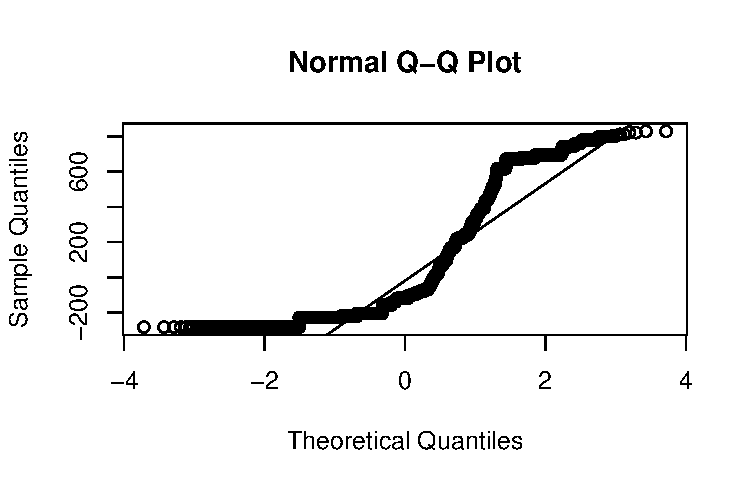
\includegraphics[width=0.6\linewidth,height=\textheight,keepaspectratio]{BCB744_Biostats_Prac_Exam_2025_files/figure-pdf/chunk17-1.pdf}
\end{center}

\begin{Shaded}
\begin{Highlighting}[]
\CommentTok{\# Homogeneity of variances}
\FunctionTok{leveneTest}\NormalTok{(weighted\_area }\SpecialCharTok{\textasciitilde{}}\NormalTok{ section, }\AttributeTok{data =}\NormalTok{ pixel\_means)}
\end{Highlighting}
\end{Shaded}

\begin{verbatim}
Levene's Test for Homogeneity of Variance (center = median)
           Df F value    Pr(>F)    
group      18   14154 < 2.2e-16 ***
      5446551                      
---
Signif. codes:  0 '***' 0.001 '**' 0.01 '*' 0.05 '.' 0.1 ' ' 1
\end{verbatim}

\begin{Shaded}
\begin{Highlighting}[]
\CommentTok{\# Residuals vs fitted}
\FunctionTok{plot}\NormalTok{(model\_5}\FloatTok{.1}\NormalTok{, }\AttributeTok{which =} \DecValTok{1}\NormalTok{)}
\end{Highlighting}
\end{Shaded}

\begin{center}
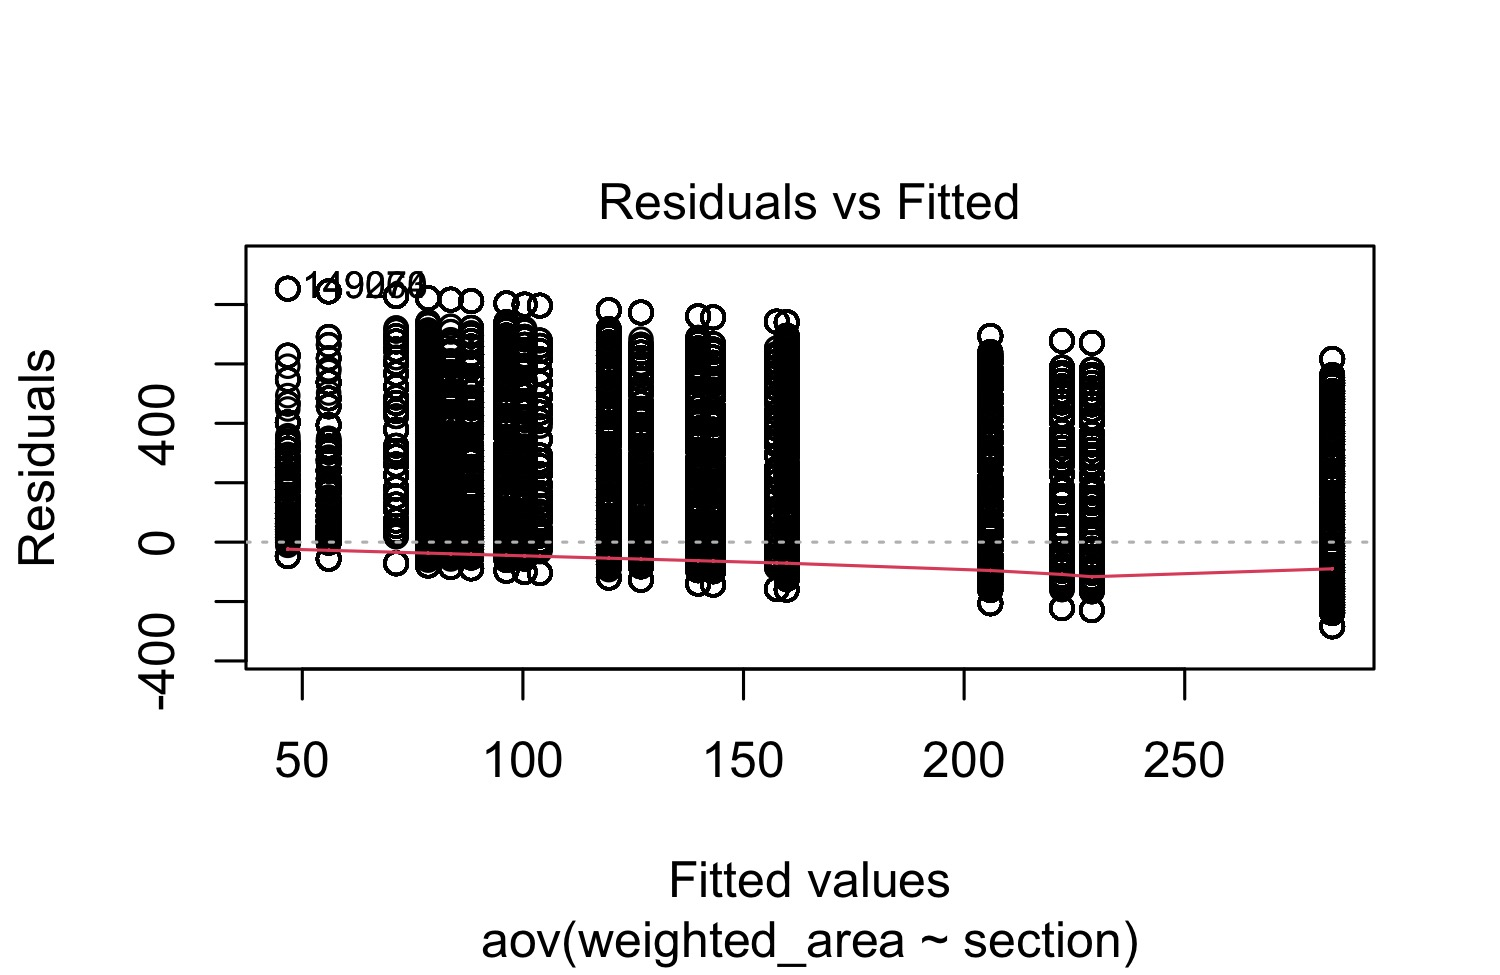
\includegraphics[width=12cm,height=\textheight,keepaspectratio]{BCB744_Biostats_Prac_Exam_2025_files/figure-pdf/chunk17-2.pdf}
\end{center}

One could do a TukeyHSD test, but the question did not explicitly ask
for this. Add two marks if correctly given and executed.

\textbf{\emph{Results}} Mean kelp canopy area varied significantly
across the 19 coastal sections assessed (F\({18,5446551}\) = 13,252,
\emph{p} \textless{} 0.001; one-way ANOVA). Residual diagnostics
indicated substantial departures from normality (Shapiro--Wilk \emph{W}
= 0.81, \emph{p} \textless{} 0.001) and non-constant variance across
groups (Levene's test: F\({18,5446551}\) = 14,154, \emph{p} \textless{}
0.001), though the extremely large sample size renders the ANOVA robust
to these violations. The fitted model accounted for a substantial
proportion of the spatial variance in kelp canopy area. Residual plots
suggested heteroscedasticity consistent with spatial heterogeneity in
canopy distributions.

To provide a fully defensible hypothesis test (considering both
assumptions were violated), do a Kruskal--Wallis rank sum test. This is
the standard non-parametric alternative to one-way ANOVA when comparing
more than two independent groups (here, coastal sections). It tests
whether the distributions of kelp canopy area differ across sections
without assuming normality or equal variances.

\subsubsection{5.2 Spatial Differences Between Biogeographical
Provinces}\label{spatial-differences-between-biogeographical-provinces}

Question: Is there a statistically significant difference in mean kelp
canopy area between biogeographical provinces?

\textbf{Answer}

Hypotheses:

\begin{itemize}
\tightlist
\item
  Null (H₀): Mean kelp canopy area is not different amongst bioregions.
\item
  Alternative (H₁): Mean kelp canopy area differs between bioregions.
\end{itemize}

Justification: Here, bioregion is treated as a categorical predictor,
suitable for a one-way ANOVA to test inter-bioregional differences. The
weighted kelp area is the continuous response variable. Assumptions of
normality and heteroscedasticity hold.

\begin{Shaded}
\begin{Highlighting}[]
\NormalTok{model\_5}\FloatTok{.2} \OtherTok{\textless{}{-}} \FunctionTok{aov}\NormalTok{(weighted\_area }\SpecialCharTok{\textasciitilde{}}\NormalTok{ bolton, }\AttributeTok{data =}\NormalTok{ pixel\_means)}
\FunctionTok{summary}\NormalTok{(model\_5}\FloatTok{.2}\NormalTok{)}
\end{Highlighting}
\end{Shaded}

\begin{verbatim}
                 Df    Sum Sq   Mean Sq F value Pr(>F)    
bolton            2 6.897e+09 3.448e+09   39585 <2e-16 ***
Residuals   5446567 4.745e+11 8.711e+04                   
---
Signif. codes:  0 '***' 0.001 '**' 0.01 '*' 0.05 '.' 0.1 ' ' 1
\end{verbatim}

\begin{Shaded}
\begin{Highlighting}[]
\CommentTok{\# Also test assumptions...}
\NormalTok{resid\_5}\FloatTok{.2} \OtherTok{\textless{}{-}} \FunctionTok{sample}\NormalTok{(}\FunctionTok{residuals}\NormalTok{(model\_5}\FloatTok{.2}\NormalTok{), }\DecValTok{5000}\NormalTok{)}

\FunctionTok{shapiro.test}\NormalTok{(resid\_5}\FloatTok{.2}\NormalTok{)}
\end{Highlighting}
\end{Shaded}

\begin{verbatim}

    Shapiro-Wilk normality test

data:  resid_5.2
W = 0.74748, p-value < 2.2e-16
\end{verbatim}

\begin{Shaded}
\begin{Highlighting}[]
\FunctionTok{qqnorm}\NormalTok{(resid\_5}\FloatTok{.2}\NormalTok{); }\FunctionTok{qqline}\NormalTok{(resid\_5}\FloatTok{.2}\NormalTok{)}
\end{Highlighting}
\end{Shaded}

\begin{center}
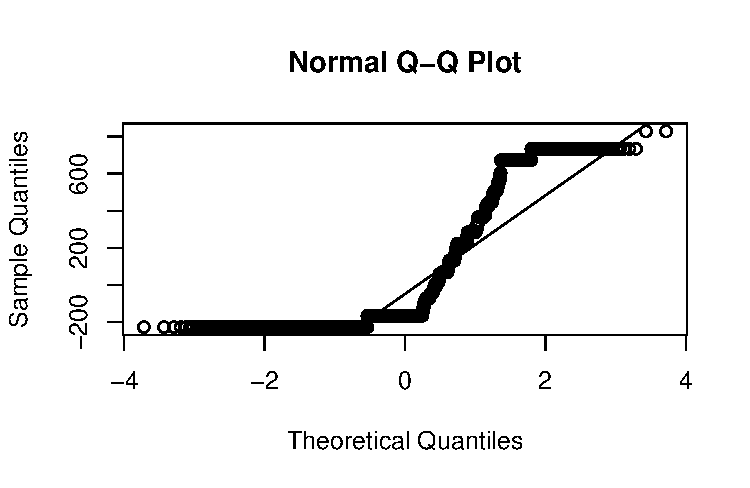
\includegraphics[width=0.6\linewidth,height=\textheight,keepaspectratio]{BCB744_Biostats_Prac_Exam_2025_files/figure-pdf/chunk18-1.pdf}
\end{center}

\begin{Shaded}
\begin{Highlighting}[]
\FunctionTok{leveneTest}\NormalTok{(weighted\_area }\SpecialCharTok{\textasciitilde{}}\NormalTok{ bolton, }\AttributeTok{data =}\NormalTok{ pixel\_means)}
\end{Highlighting}
\end{Shaded}

\begin{verbatim}
Levene's Test for Homogeneity of Variance (center = median)
           Df F value    Pr(>F)    
group       2   39585 < 2.2e-16 ***
      5446567                      
---
Signif. codes:  0 '***' 0.001 '**' 0.01 '*' 0.05 '.' 0.1 ' ' 1
\end{verbatim}

\begin{Shaded}
\begin{Highlighting}[]
\FunctionTok{plot}\NormalTok{(model\_5}\FloatTok{.2}\NormalTok{, }\AttributeTok{which =} \DecValTok{1}\NormalTok{)}
\end{Highlighting}
\end{Shaded}

\begin{center}
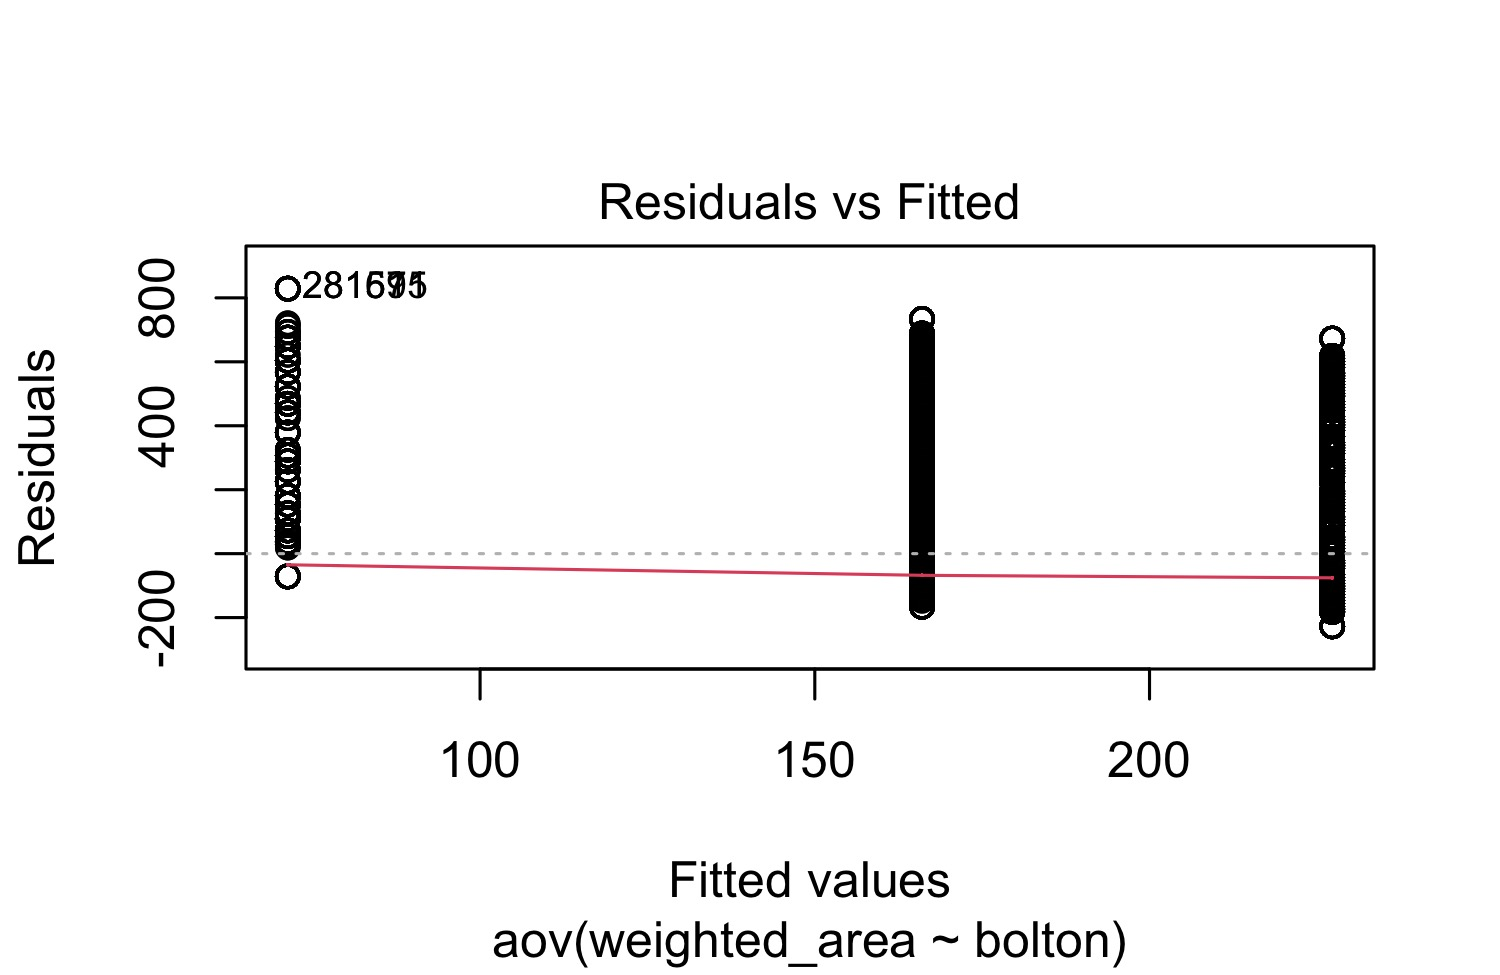
\includegraphics[width=12cm,height=\textheight,keepaspectratio]{BCB744_Biostats_Prac_Exam_2025_files/figure-pdf/chunk18-2.pdf}
\end{center}

\textbf{\emph{Results}} A one-way ANOVA revealed significant differences
in mean kelp canopy area between the three biogeographical provinces
(BMP, SWP, AMP) (F\({2,5446567}\) = 39,585, \emph{p} \textless{} 0.001).
Residual analysis again revealed non-normal error distribution
(Shapiro--Wilk \emph{W} = 0.75, \emph{p} \textless{} 0.001) and unequal
variances among provinces (Levene's test: F\({2,5446567}\) = 39,585,
\emph{p} \textless{} 0.001). Despite these assumption violations, the
effect was large and consistent with substantial regional
differentiation in canopy extent. Residuals from the model were
symmetrically distributed but with longer tails in high-variance
provinces.

As before, a Kruskal--Wallis rank sum test is recommended. Again
suitable, since the bioregion variable has three independent levels.
This test evaluates whether the central tendency of canopy area differs
among provinces without assuming parametric conditions.

\subsubsection{5.3 Interaction Between Section and
Province}\label{interaction-between-section-and-province}

Question: Is there an interaction between coastal section and
biogeographical province in explaining variation in kelp canopy area?

\textbf{Answer}

Hypotheses:

\begin{itemize}
\tightlist
\item
  H₀₁ (Main effect -- Section): There are no differences in mean kelp
  canopy area across coastal sections.
\item
  H₀₂ (Main effect -- Province): There are no differences in mean kelp
  canopy area across biogeographical provinces.
\item
  H₀₃ (Interaction): The effect of coastal section on kelp canopy area
  is the same across all provinces (i.e., no interaction).
\item
  H₁ (Alternative): At least one main effect is non-zero, or there is a
  significant interaction (i.e., the influence of section depends on the
  province).
\end{itemize}

A two-way ANOVA with interaction is appropriate here because:

\begin{itemize}
\tightlist
\item
  Both predictors, i.e., \texttt{section} (a factor) and province
  (\texttt{bolton}, also a factor), are categorical.
\item
  The response variable (\texttt{weighted\_area}) is continuous and
  assumed to meet the assumptions of normality and homogeneity of
  variance.
\item
  The interaction term allows us to assess whether the spatial
  granularity of section varies in importance across broader-scale
  bioregions.
\end{itemize}

This model allows us to partition variation in canopy area into
hierarchical (or cross-cutting) spatial components.

\begin{Shaded}
\begin{Highlighting}[]
\CommentTok{\# Two{-}way ANOVA with interaction}
\NormalTok{model\_5}\FloatTok{.3} \OtherTok{\textless{}{-}} \FunctionTok{aov}\NormalTok{(weighted\_area }\SpecialCharTok{\textasciitilde{}}\NormalTok{ section }\SpecialCharTok{*}\NormalTok{ bolton, }\AttributeTok{data =}\NormalTok{ pixel\_means)}

\CommentTok{\# Summary of the model}
\FunctionTok{summary}\NormalTok{(model\_5}\FloatTok{.3}\NormalTok{)}
\end{Highlighting}
\end{Shaded}

\begin{verbatim}
                 Df    Sum Sq   Mean Sq F value Pr(>F)    
section          18 2.020e+10 1.122e+09   13252 <2e-16 ***
Residuals   5446551 4.612e+11 8.467e+04                   
---
Signif. codes:  0 '***' 0.001 '**' 0.01 '*' 0.05 '.' 0.1 ' ' 1
\end{verbatim}

\begin{Shaded}
\begin{Highlighting}[]
\CommentTok{\# Also test assumptions...}
\NormalTok{resid\_5}\FloatTok{.3} \OtherTok{\textless{}{-}} \FunctionTok{sample}\NormalTok{(}\FunctionTok{residuals}\NormalTok{(model\_5}\FloatTok{.3}\NormalTok{), }\DecValTok{5000}\NormalTok{)}

\FunctionTok{shapiro.test}\NormalTok{(resid\_5}\FloatTok{.3}\NormalTok{)}
\end{Highlighting}
\end{Shaded}

\begin{verbatim}

    Shapiro-Wilk normality test

data:  resid_5.3
W = 0.81015, p-value < 2.2e-16
\end{verbatim}

\begin{Shaded}
\begin{Highlighting}[]
\FunctionTok{qqnorm}\NormalTok{(resid\_5}\FloatTok{.3}\NormalTok{); }\FunctionTok{qqline}\NormalTok{(resid\_5}\FloatTok{.3}\NormalTok{)}
\end{Highlighting}
\end{Shaded}

\begin{center}
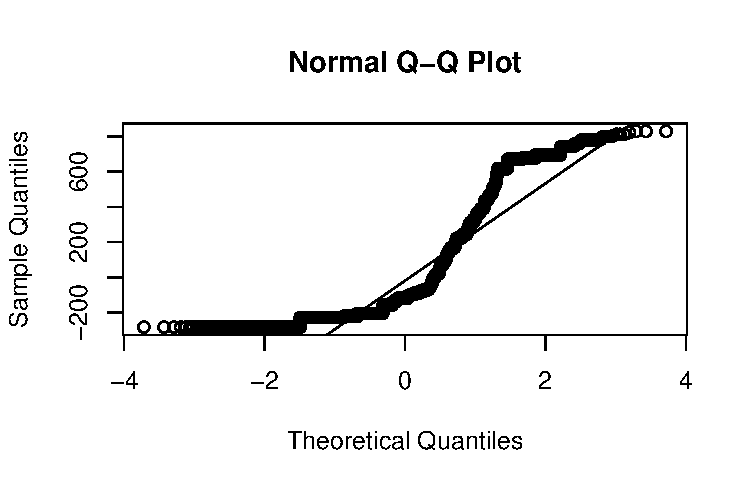
\includegraphics[width=0.6\linewidth,height=\textheight,keepaspectratio]{BCB744_Biostats_Prac_Exam_2025_files/figure-pdf/chunk19-1.pdf}
\end{center}

\begin{Shaded}
\begin{Highlighting}[]
\NormalTok{car}\SpecialCharTok{::}\FunctionTok{leveneTest}\NormalTok{(model\_5}\FloatTok{.3}\NormalTok{)}
\end{Highlighting}
\end{Shaded}

\begin{verbatim}
Levene's Test for Homogeneity of Variance (center = median)
           Df F value    Pr(>F)    
group      18   14154 < 2.2e-16 ***
      5446551                      
---
Signif. codes:  0 '***' 0.001 '**' 0.01 '*' 0.05 '.' 0.1 ' ' 1
\end{verbatim}

\begin{Shaded}
\begin{Highlighting}[]
\FunctionTok{plot}\NormalTok{(model\_5}\FloatTok{.3}\NormalTok{, }\AttributeTok{which =} \DecValTok{1}\NormalTok{)}
\end{Highlighting}
\end{Shaded}

\begin{center}
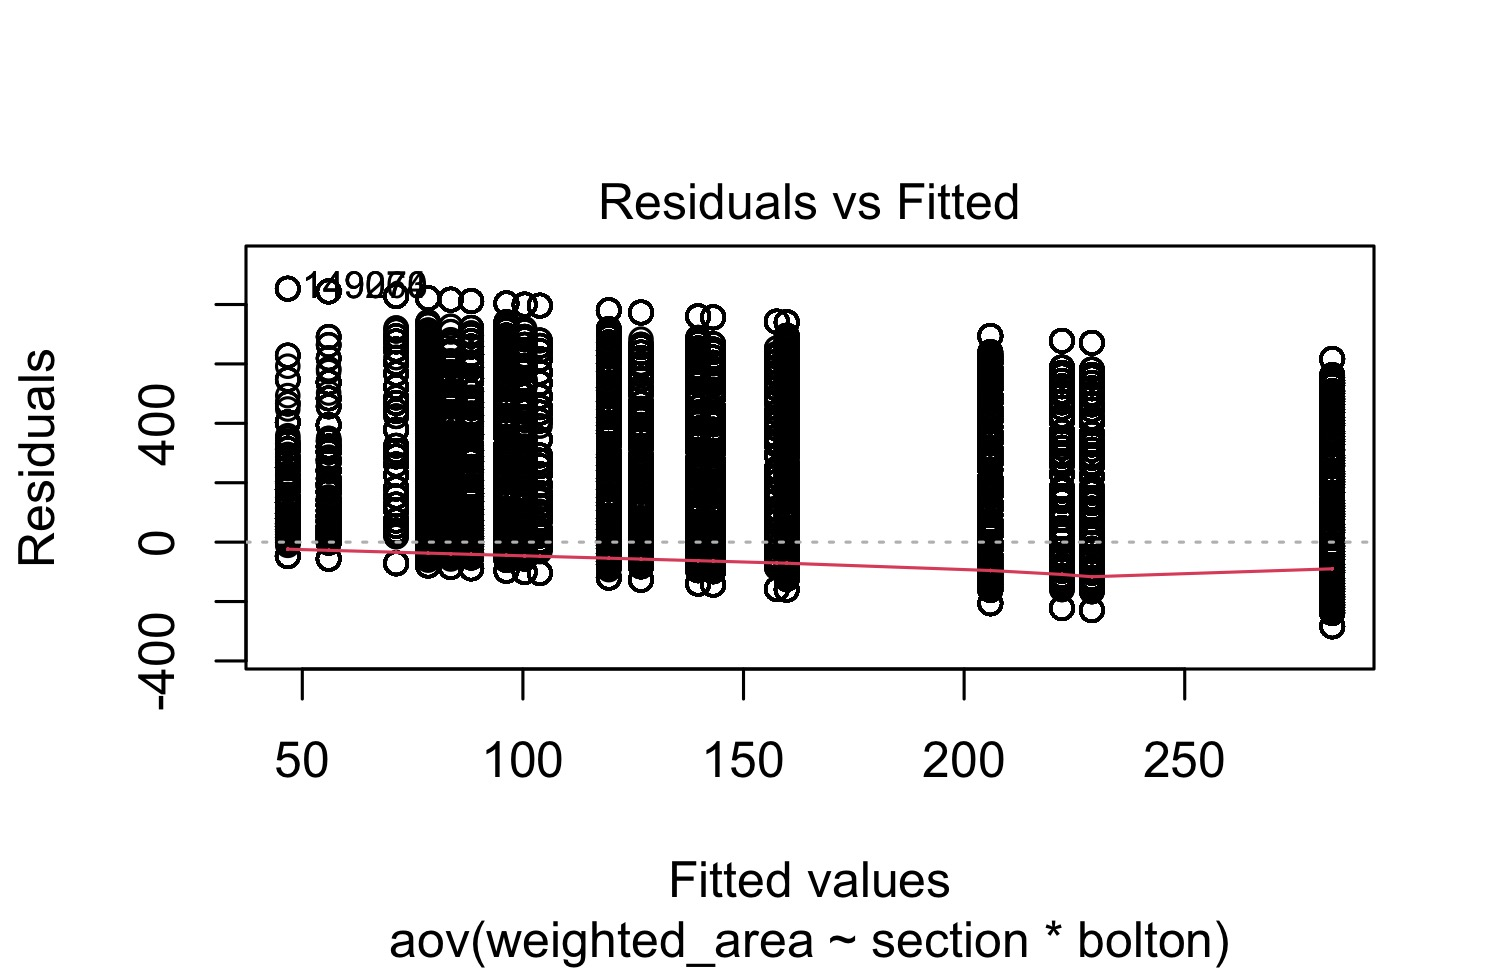
\includegraphics[width=12cm,height=\textheight,keepaspectratio]{BCB744_Biostats_Prac_Exam_2025_files/figure-pdf/chunk19-2.pdf}
\end{center}

In this case, interaction terms cannot be estimated, because there's no
shared replication across bioregions within sections. The design is not
factorial. The solution is to fix mixed models with random and fixed
effects.

\textbf{\emph{Results}} A two-way ANOVA incorporating both section and
biogeographical province, including their interaction, confirmed strong
spatial structuring of kelp canopy area (F\(_{18,5446551}\) = 13,252,
\emph{p} \textless{} 0.001 for the section main effect). However, the
interaction term was non-estimable due to the confounded structure of
the design --- each section belonged uniquely to a single province,
precluding factorial replication. As such, a fully crossed design could
not be evaluated within a fixed-effects ANOVA framework. Model residuals
displayed similar deviations from normality and homogeneity as in
previous analyses, but were centered and broadly symmetric.

A non-parametric two-way tests for interaction effects do not exist.
Because of the nested design, a fully non-parametric two-way ANOVA is
not viable. As an alternative approach, perform separate Kruskal--Wallis
tests within each province, or apply a permutation-based two-way ANOVA
that accommodates unbalanced and non-normal designs.

\subsubsection{5.4 Linear Trend Over Time by
Province}\label{linear-trend-over-time-by-province}

Question: Is there a linear trend in kelp canopy area over time, and
does the direction or strength of this trend differ between
biogeographical provinces?

\textbf{Answer}

Hypotheses:

\begin{itemize}
\tightlist
\item
  H₀₁ (Main effect of time): There is no linear trend in kelp canopy
  area over time.
\item
  H₀₂ (Time × Province interaction): The effect (slope) of year is the
  same across all provinces.
\item
  H₁ (Alternative): Kelp canopy area shows a linear trend over time, and
  the rate or direction of change differs by province.
\end{itemize}

This is a typical ANCOVA design because:

\begin{itemize}
\tightlist
\item
  The continuous predictor \texttt{year} captures temporal trends.
\item
  The categorical predictor \texttt{bolton} accounts for regional
  differences.
\item
  The interaction term \texttt{year} × \texttt{bolton} assesses whether
  temporal slopes differ among provinces.
\end{itemize}

ANCOVA is ideal for testing whether regression lines have the same slope
across groups; here, whether kelp decline/growth rates differ by
province.

\begin{Shaded}
\begin{Highlighting}[]
\CommentTok{\# Aggregate by year and province}
\NormalTok{province\_annual }\OtherTok{\textless{}{-}}\NormalTok{ pixel\_means }\SpecialCharTok{|\textgreater{}}
  \FunctionTok{group\_by}\NormalTok{(year, bolton) }\SpecialCharTok{|\textgreater{}}
  \FunctionTok{summarise}\NormalTok{(}\AttributeTok{mean\_area =} \FunctionTok{mean}\NormalTok{(weighted\_area, }\AttributeTok{na.rm =} \ConstantTok{TRUE}\NormalTok{), }\AttributeTok{.groups =} \StringTok{"drop"}\NormalTok{)}

\CommentTok{\# Fit the ANCOVA model}
\NormalTok{model\_5}\FloatTok{.4} \OtherTok{\textless{}{-}} \FunctionTok{lm}\NormalTok{(mean\_area }\SpecialCharTok{\textasciitilde{}}\NormalTok{ year }\SpecialCharTok{*}\NormalTok{ bolton, }\AttributeTok{data =}\NormalTok{ province\_annual)}

\CommentTok{\# Summary of model}
\CommentTok{\# summary(model\_5.4)  \# Dont print... too long!}

\CommentTok{\# A Type III ANOVA, as in the car::Anova() function with type = 3, tests the}
\CommentTok{\# significance of each effect after accounting for all other effects in the}
\CommentTok{\# model, including interactions. It asks: “What is the unique contribution}
\CommentTok{\# of this factor, given that all others (including interactions) are already}
\CommentTok{\# in the model?”}
\FunctionTok{Anova}\NormalTok{(model\_5}\FloatTok{.4}\NormalTok{, }\AttributeTok{type =} \DecValTok{3}\NormalTok{)}
\end{Highlighting}
\end{Shaded}

\begin{verbatim}
Anova Table (Type III tests)

Response: mean_area
            Sum Sq  Df F value    Pr(>F)    
(Intercept) 125927   1 45.2807 6.830e-10 ***
year        127296   1 45.7731 5.702e-10 ***
bolton       38795   2  6.9749  0.001379 ** 
year:bolton  37570   2  6.7548  0.001679 ** 
Residuals   322599 116                      
---
Signif. codes:  0 '***' 0.001 '**' 0.01 '*' 0.05 '.' 0.1 ' ' 1
\end{verbatim}

\begin{Shaded}
\begin{Highlighting}[]
\FunctionTok{ggplot}\NormalTok{(province\_annual,}
       \FunctionTok{aes}\NormalTok{(}\AttributeTok{x =}\NormalTok{ year, }\AttributeTok{y =}\NormalTok{ mean\_area, }\AttributeTok{color =}\NormalTok{ bolton)) }\SpecialCharTok{+}
  \FunctionTok{geom\_point}\NormalTok{(}\AttributeTok{alpha =} \FloatTok{0.4}\NormalTok{) }\SpecialCharTok{+}
  \FunctionTok{geom\_smooth}\NormalTok{(}\AttributeTok{method =} \StringTok{"lm"}\NormalTok{, }\AttributeTok{se =} \ConstantTok{FALSE}\NormalTok{) }\SpecialCharTok{+}
  \FunctionTok{theme\_minimal}\NormalTok{() }\SpecialCharTok{+}
  \FunctionTok{labs}\NormalTok{(}
    \AttributeTok{title =} \StringTok{"Linear Trends in Kelp Canopy Area by Province"}\NormalTok{,}
    \AttributeTok{y =} \StringTok{"Mean Canopy Area per Pixel"}\NormalTok{,}
    \AttributeTok{x =} \StringTok{"Year"}
\NormalTok{  )}
\end{Highlighting}
\end{Shaded}

\begin{center}
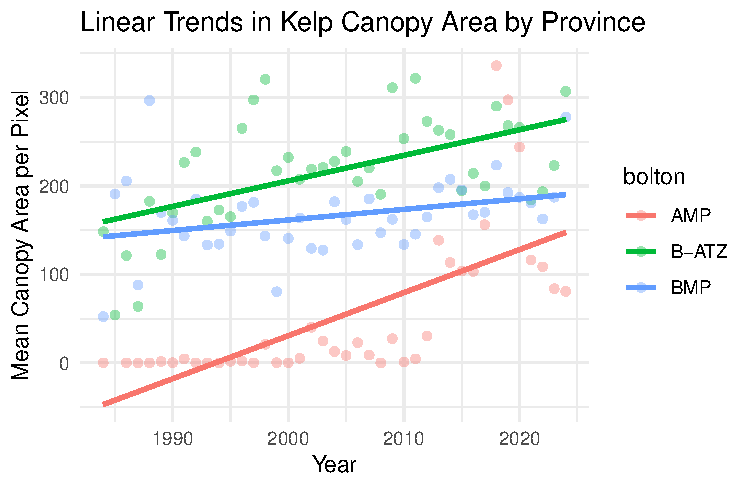
\includegraphics[width=0.6\linewidth,height=\textheight,keepaspectratio]{BCB744_Biostats_Prac_Exam_2025_files/figure-pdf/chunk20-1.pdf}
\end{center}

\begin{Shaded}
\begin{Highlighting}[]
\CommentTok{\# Also test assumptions...}
\NormalTok{resid\_5}\FloatTok{.4} \OtherTok{\textless{}{-}} \FunctionTok{residuals}\NormalTok{(model\_5}\FloatTok{.4}\NormalTok{)}

\CommentTok{\# Normality}
\FunctionTok{shapiro.test}\NormalTok{(resid\_5}\FloatTok{.4}\NormalTok{)}
\end{Highlighting}
\end{Shaded}

\begin{verbatim}

    Shapiro-Wilk normality test

data:  resid_5.4
W = 0.93452, p-value = 1.599e-05
\end{verbatim}

\begin{Shaded}
\begin{Highlighting}[]
\FunctionTok{qqnorm}\NormalTok{(resid\_5}\FloatTok{.4}\NormalTok{); }\FunctionTok{qqline}\NormalTok{(resid\_5}\FloatTok{.4}\NormalTok{)}
\end{Highlighting}
\end{Shaded}

\begin{center}
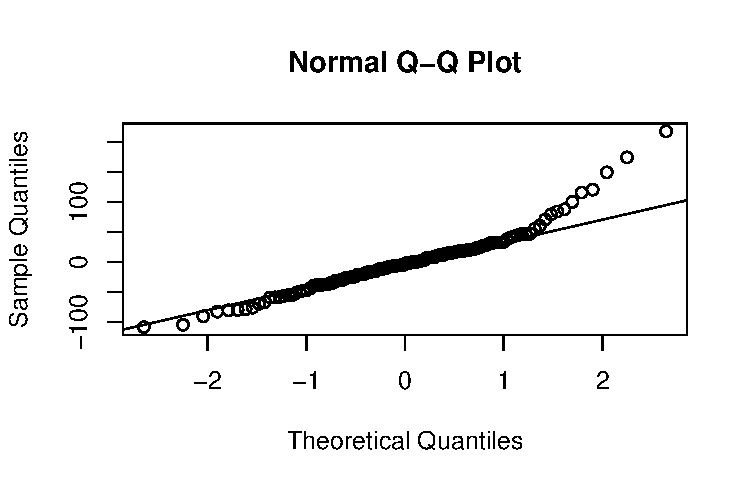
\includegraphics[width=12cm,height=\textheight,keepaspectratio]{BCB744_Biostats_Prac_Exam_2025_files/figure-pdf/chunk20-2.pdf}
\end{center}

\begin{Shaded}
\begin{Highlighting}[]
\CommentTok{\# Homoscedasticity}
\FunctionTok{plot}\NormalTok{(model\_5}\FloatTok{.4}\NormalTok{, }\AttributeTok{which =} \DecValTok{1}\NormalTok{)}
\end{Highlighting}
\end{Shaded}

\begin{center}
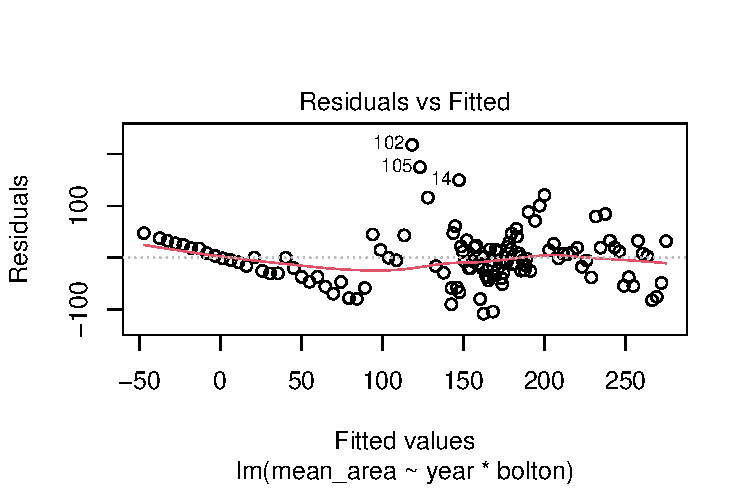
\includegraphics[width=0.6\linewidth,height=\textheight,keepaspectratio]{BCB744_Biostats_Prac_Exam_2025_files/figure-pdf/chunk20-3.pdf}
\end{center}

\begin{Shaded}
\begin{Highlighting}[]
\FunctionTok{bptest}\NormalTok{(model\_5}\FloatTok{.4}\NormalTok{)  }\CommentTok{\# Breusch{-}Pagan test or any other suitable test}
\end{Highlighting}
\end{Shaded}

\begin{verbatim}

    studentized Breusch-Pagan test

data:  model_5.4
BP = 16.228, df = 5, p-value = 0.006223
\end{verbatim}

\begin{Shaded}
\begin{Highlighting}[]
\CommentTok{\# Multicollinearity}
\CommentTok{\# Don\textquotesingle{}t penalise students for not testing multicollinearity, but}
\CommentTok{\# add a bonus two marks if included}
\FunctionTok{vif}\NormalTok{(model\_5}\FloatTok{.4}\NormalTok{)}
\end{Highlighting}
\end{Shaded}

\begin{verbatim}
                    GVIF Df GVIF^(1/(2*Df))
year        3.138942e+00  1        1.771706
bolton      8.468999e+08  2      170.591747
year:bolton 8.466877e+08  2      170.581063
\end{verbatim}

\begin{Shaded}
\begin{Highlighting}[]
\CommentTok{\# Independence of residuals}
\FunctionTok{dwtest}\NormalTok{(model\_5}\FloatTok{.4}\NormalTok{)  }\CommentTok{\# Durbin{-}Watson test}
\end{Highlighting}
\end{Shaded}

\begin{verbatim}

    Durbin-Watson test

data:  model_5.4
DW = 1.7605, p-value = 0.1114
alternative hypothesis: true autocorrelation is greater than 0
\end{verbatim}

\textbf{\emph{Results}} The ANCOVA model indicated a significant linear
increase in mean kelp canopy area over time across all provinces
(F\({1,116}\) = 45.8, \emph{p} \textless{} 0.001), with significant
differences in temporal trends among provinces (year × province
interaction: F\({2,116}\) = 6.75, \emph{p} = 0.0017). This suggests that
both the direction and magnitude of temporal trends in canopy area are
modulated by biogeographical province. Residuals exhibited slight
right-skew (Shapiro--Wilk \emph{W} = 0.93, \emph{p} \textless{} 0.001),
and heteroscedasticity was supported by a significant Breusch--Pagan
test (BP = 16.23, df = 5, \emph{p} = 0.006). No evidence of residual
autocorrelation was detected (Durbin--Watson DW = 1.76, \emph{p} =
0.11). Variance inflation factors indicated high collinearity between
province and interaction terms, reflecting the nested structure of the
provinces over time.

Pragmatic alternative to account for non-normality, heteroscedasticity,
and collinearity: perform separate Spearman's rank correlation tests
between year and mean area within each province to assess monotonic
trends, then compare slope magnitudes informally or using non-parametric
trend tests like Mann--Kendall.

\subsubsection{5.5 Seasonal Variation Across
Provinces}\label{seasonal-variation-across-provinces}

Question: Does the seasonal pattern in kelp canopy area differ between
provinces?

\textbf{Answer}

Hypotheses:

\begin{itemize}
\tightlist
\item
  H₀₁ (Main effect of quarter): Mean kelp canopy area does not vary
  across seasons (quarters).
\item
  H₀₂ (Quarter × Province interaction): The pattern of seasonal
  variation is the same in all provinces --- i.e., there is no
  interaction.
\item
  H₁ (Alternative): There are seasonal differences in kelp canopy area,
  and the shape or magnitude of the seasonal cycle differs by province.
\end{itemize}

A two-way ANOVA is appropriate here, with:

\begin{itemize}
\tightlist
\item
  \texttt{quarter} as a categorical predictor representing seasonal
  variation.
\item
  \texttt{bolton} as a categorical grouping variable for province.
\item
  An interaction term (\texttt{quarter} × \texttt{bolton}) to test
  whether seasonal cycles differ by region.
\end{itemize}

This model assesses both the amplitude and phase-shift of seasonal
dynamics across spatial domains.

\begin{Shaded}
\begin{Highlighting}[]
\CommentTok{\# Ensure quarter is treated as a categorical variable}
\NormalTok{pixel\_means }\OtherTok{\textless{}{-}}\NormalTok{ pixel\_means }\SpecialCharTok{|\textgreater{}}
  \FunctionTok{mutate}\NormalTok{(}\AttributeTok{quarter =} \FunctionTok{as.factor}\NormalTok{(quarter))}

\CommentTok{\# Group by year, quarter, and province to retain replication across years}
\NormalTok{province\_seasonal\_replicated }\OtherTok{\textless{}{-}}\NormalTok{ pixel\_means }\SpecialCharTok{|\textgreater{}}
  \FunctionTok{group\_by}\NormalTok{(year, quarter, bolton) }\SpecialCharTok{|\textgreater{}}
  \FunctionTok{summarise}\NormalTok{(}\AttributeTok{mean\_area =} \FunctionTok{mean}\NormalTok{(weighted\_area, }\AttributeTok{na.rm =} \ConstantTok{TRUE}\NormalTok{), }\AttributeTok{.groups =} \StringTok{"drop"}\NormalTok{)}

\CommentTok{\# Fit two{-}way ANOVA with interaction}
\NormalTok{model\_5}\FloatTok{.5} \OtherTok{\textless{}{-}} \FunctionTok{aov}\NormalTok{(mean\_area }\SpecialCharTok{\textasciitilde{}}\NormalTok{ quarter }\SpecialCharTok{*}\NormalTok{ bolton, }\AttributeTok{data =}\NormalTok{ province\_seasonal\_replicated)}

\CommentTok{\# Model summary}
\FunctionTok{summary}\NormalTok{(model\_5}\FloatTok{.5}\NormalTok{)}
\end{Highlighting}
\end{Shaded}

\begin{verbatim}
                Df  Sum Sq Mean Sq F value Pr(>F)    
quarter          3   66835   22278   3.061 0.0281 *  
bolton           2 1944753  972377 133.590 <2e-16 ***
quarter:bolton   6  103175   17196   2.362 0.0295 *  
Residuals      423 3078948    7279                   
---
Signif. codes:  0 '***' 0.001 '**' 0.01 '*' 0.05 '.' 0.1 ' ' 1
\end{verbatim}

\begin{Shaded}
\begin{Highlighting}[]
\CommentTok{\# Extract residuals}
\NormalTok{resid\_5}\FloatTok{.5} \OtherTok{\textless{}{-}} \FunctionTok{residuals}\NormalTok{(model\_5}\FloatTok{.5}\NormalTok{)}

\CommentTok{\# Test for normality of residuals}
\FunctionTok{shapiro.test}\NormalTok{(resid\_5}\FloatTok{.5}\NormalTok{)}
\end{Highlighting}
\end{Shaded}

\begin{verbatim}

    Shapiro-Wilk normality test

data:  resid_5.5
W = 0.95331, p-value = 1.7e-10
\end{verbatim}

\begin{Shaded}
\begin{Highlighting}[]
\FunctionTok{qqnorm}\NormalTok{(resid\_5}\FloatTok{.5}\NormalTok{); }\FunctionTok{qqline}\NormalTok{(resid\_5}\FloatTok{.5}\NormalTok{)}
\end{Highlighting}
\end{Shaded}

\begin{center}
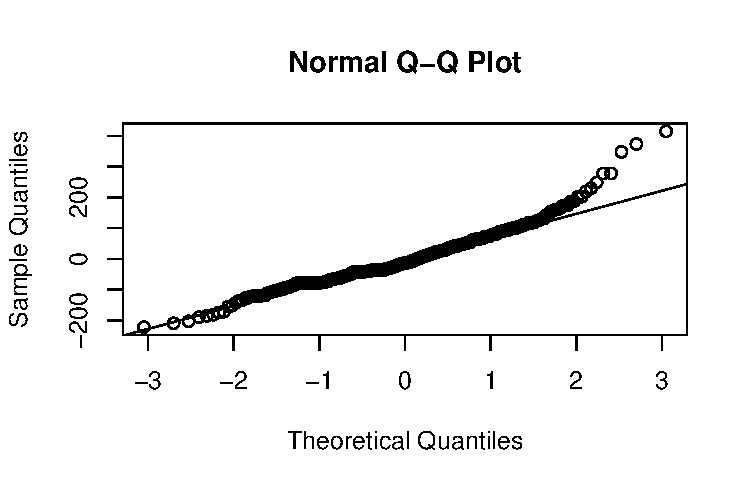
\includegraphics[width=0.6\linewidth,height=\textheight,keepaspectratio]{BCB744_Biostats_Prac_Exam_2025_files/figure-pdf/chunk21-1.pdf}
\end{center}

\begin{Shaded}
\begin{Highlighting}[]
\CommentTok{\# Test for homogeneity of variances across quarter × province combinations}
\NormalTok{province\_seasonal\_replicated}\SpecialCharTok{$}\NormalTok{group }\OtherTok{\textless{}{-}} \FunctionTok{interaction}\NormalTok{(province\_seasonal\_replicated}\SpecialCharTok{$}\NormalTok{quarter,}
\NormalTok{                                                  province\_seasonal\_replicated}\SpecialCharTok{$}\NormalTok{bolton)}
\FunctionTok{leveneTest}\NormalTok{(mean\_area }\SpecialCharTok{\textasciitilde{}}\NormalTok{ group, }\AttributeTok{data =}\NormalTok{ province\_seasonal\_replicated)}
\end{Highlighting}
\end{Shaded}

\begin{verbatim}
Levene's Test for Homogeneity of Variance (center = median)
       Df F value   Pr(>F)   
group  11  2.3599 0.007804 **
      423                    
---
Signif. codes:  0 '***' 0.001 '**' 0.01 '*' 0.05 '.' 0.1 ' ' 1
\end{verbatim}

\begin{Shaded}
\begin{Highlighting}[]
\CommentTok{\# Interaction plot: mean kelp canopy area by quarter and province}
\FunctionTok{ggplot}\NormalTok{(province\_seasonal\_replicated,}
                           \FunctionTok{aes}\NormalTok{(}\AttributeTok{x =}\NormalTok{ quarter,}
                               \AttributeTok{y =}\NormalTok{ mean\_area,}
                               \AttributeTok{group =}\NormalTok{ bolton,}
                               \AttributeTok{color =}\NormalTok{ bolton)) }\SpecialCharTok{+}
  \FunctionTok{stat\_summary}\NormalTok{(}\AttributeTok{fun =}\NormalTok{ mean, }\AttributeTok{geom =} \StringTok{"line"}\NormalTok{, }\AttributeTok{size =} \DecValTok{1}\NormalTok{) }\SpecialCharTok{+}
  \FunctionTok{stat\_summary}\NormalTok{(}\AttributeTok{fun =}\NormalTok{ mean, }\AttributeTok{geom =} \StringTok{"point"}\NormalTok{, }\AttributeTok{size =} \DecValTok{2}\NormalTok{) }\SpecialCharTok{+}
  \FunctionTok{theme\_minimal}\NormalTok{(}\AttributeTok{base\_size =} \DecValTok{11}\NormalTok{) }\SpecialCharTok{+}
  \FunctionTok{scale\_x\_discrete}\NormalTok{(}\AttributeTok{labels =} \FunctionTok{c}\NormalTok{(}\StringTok{"Q1"}\NormalTok{, }\StringTok{"Q2"}\NormalTok{, }\StringTok{"Q3"}\NormalTok{, }\StringTok{"Q4"}\NormalTok{)) }\SpecialCharTok{+}
  \FunctionTok{labs}\NormalTok{(}
    \AttributeTok{title =} \StringTok{"Interaction of Quarter and Province on Mean Kelp Canopy Area"}\NormalTok{,}
    \AttributeTok{x =} \StringTok{"Quarter"}\NormalTok{,}
    \AttributeTok{y =} \StringTok{"Mean Kelp Canopy Area (per pixel per year)"}\NormalTok{,}
    \AttributeTok{color =} \StringTok{"Province"}
\NormalTok{  ) }\SpecialCharTok{+}
  \FunctionTok{theme}\NormalTok{(}\AttributeTok{legend.position =} \StringTok{"bottom"}\NormalTok{)}
\end{Highlighting}
\end{Shaded}

\begin{center}
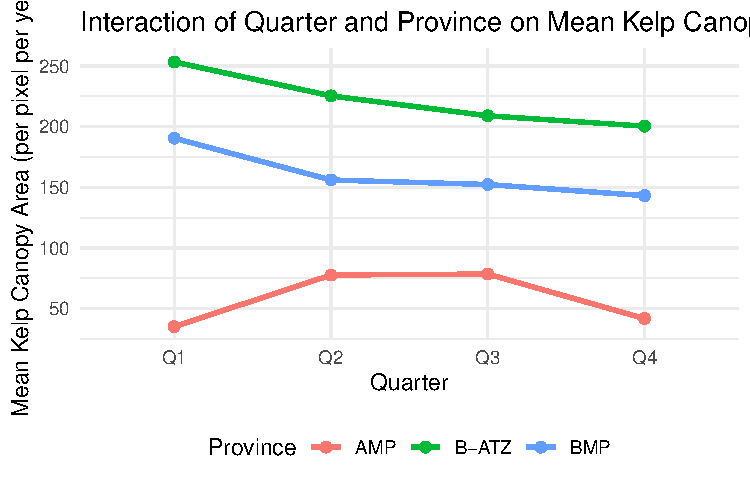
\includegraphics[width=12cm,height=\textheight,keepaspectratio]{BCB744_Biostats_Prac_Exam_2025_files/figure-pdf/chunk21-2.pdf}
\end{center}

\textbf{\emph{Results}} Seasonal variation in kelp canopy area differed
significantly among provinces (two-way ANOVA: quarter × province
interaction: F\({6,423}\) = 2.36, p = 0.030). Both main effects were
significant, with variation among quarters (F\({3,423}\) = 3.06,
\emph{p} = 0.028) and among provinces (F\({2,423}\) = 133.6, \emph{p}
\textless{} 0.001). Residuals exhibited mild non-normality
(Shapiro--Wilk \emph{W} = 0.95, \emph{p} \textless{} 0.001), and
homoscedasticity was violated across the interaction groups (Levene's
test: F\({11,423}\) = 2.36, \emph{p} = 0.008). Nevertheless, interaction
plots indicated province-specific seasonal cycles in canopy area that
were consistent across years.

There is no easy non-parametric alternative.

\subsubsection{General Instructions for Task 5
(above)}\label{general-instructions-for-task-5-above}

For each sub-question, above, consider:

\begin{itemize}
\tightlist
\item
  formally state the null and alternative hypotheses;
\item
  justify your choice of model;
\item
  justify your choice of predictors;
\item
  justify your decision to aggregate or not aggregate the data at
  various levels;
\item
  discuss the assumptions involved and any violations you detect;
\item
  present the relevant model outputs and statistical tests;
\item
  include visualisations where appropriate (e.g.~interaction plots,
  trend lines, diagnostic plots);
\item
  justify your choice of visualisation; and
\item
  present the results in a clear and concise manner, including tables
  and figures where appropriate, in a manner that would be appropriate
  for a scientific audience (e.g.~a journal article).
\end{itemize}

You are not required to use the same modelling approach for all five
sub-questions, though consistency across related questions is
encouraged.

\subsection{Task 6: Write-up}\label{task-6-write-up}

\begin{itemize}
\tightlist
\item
  \textbf{{[}Task Weight: 10\%{]}}
\end{itemize}

Write a short report (maximum 2 pages of text) that synthesises your
findings across Tasks 2 through 5. This report should be written in the
style of the Discussion section of a scientific paper, intended for an
ecological audience.

Your goal is to interpret the major patterns and relationships you have
identified, and to comment meaningfully on their ecological
significance. Your write-up should include:

\begin{itemize}
\tightlist
\item
  Temporal Trends and Seasonality.
\item
  Spatial Structure and Biogeography.
\item
  Interaction Effects and Spatial--Temporal Coupling.
\item
  Limitations and Assumptions.
\item
  Ecological Interpretation.
\end{itemize}

Format and tone:

\begin{itemize}
\tightlist
\item
  Aim for clarity and economy of expression.
\item
  Don't generate any new tables and figures. The tables and figures from
  Tasks 2 through 5 should be sufficient.
\item
  Write in complete paragraphs. Avoid bulleted summaries.
\item
  Add references to the tables and figures from Tasks 2 through 5 as
  needed.
\item
  Cite any additional references you use.
\end{itemize}

\textbf{Answer}

\textbf{\emph{Note to Assessor:}} Penalise all text that was clearly AI
generated by subtracting 50\% off the mark.

\emph{Discussion}

Our analysis of long-term kelp canopy dynamics revealed strong
spatio-temporal structuring in both the mean extent and variability of
kelp forests across southern Africa. While the limitations of simple
linear and ANOVA-based models prevent exhaustive ecological inference,
the results consistently support our observations that kelp canopy cover
is not uniformly variable in space or time, but instead shaped by
regionally distinct seasonal regimes and long-term trends that interact
with the underlying biogeographic patterns.

At the broadest temporal scale, the annual means (Task 2) show evidence
for a long-term linear increase in kelp canopy area across the study
period, although the strength and direction of this trend varied
substantially by biogeographical province. The Benguela Marine Province
(BMP) exhibited a relatively strong positive trend, while the Agulhas
and Benguela-Agulhas Transition Zone (AMP and B-ATZ) showed weaker or
inconsistent trajectories. These patterns likely reflect contrasting
oceanographic influences, specifically the differing degrees of
upwelling intensity and sea surface temperature variability across
provinces. When the annual trends were disaggregated seasonally (Task
3), the signal became more complex. Seasonal means indicated a marked
peak in kelp canopy area during austral summer and early autumn
(quarters 1 and 2). This seasonal cycle was most pronounced in BMP, less
so in B-ATZ, and relatively flat in AMP, suggesting that regional
exposure to storm-driven disturbance, solar irradiance, or herbivore
activity may modulate canopy recovery and loss at intra-annual scales.

Spatial patterns in kelp canopy extent, assessed both at the bioregional
level (Task 4.1) and at the finer spatial resolution of coastal sections
(Task 5.1), reinforce the view that biogeographic context is a dominant
driver of canopy variability. A large proportion of the overall variance
in canopy area was attributable to differences among sections, but these
differences were nested within broader provincial contrasts. The one-way
and two-way ANOVAs demonstrated strong main effects of both spatial
variables, although the interaction between section and province could
not be statistically partitioned due to their hierarchical structure.
Nonetheless, the magnitude of spatial variation suggests that local
environmental factors (such as wave exposure, topographic complexity,
and nutrient availability) likely modulate kelp dynamics on
sub-provincial scales, even as broader provincial regimes exert
overarching influence.

Where temporal and spatial effects intersect, the coupling of seasonal
cycles with regional identity becomes ecologically meaningful. Task 5.5
illustrated this clearly: although all provinces experience some degree
of seasonal fluctuation, the shape and amplitude of these cycles
differed significantly. The interaction effect between quarter and
province was significant despite the relatively simple model structure,
indicating that the timing of canopy peaks and troughs is not
synchronised coast-wide. This asynchrony complicates large-scale
generalisations about kelp seasonality and underscores the importance of
considering regional context in ecological forecasting. That the BMP,
for instance, displays both the strongest seasonal cycle and the most
pronounced long-term increase suggests a possible reinforcing
interaction between natural seasonal pulses and long-term drivers such
as ocean cooling (prevalent in the kelp's distributional range) or
changing storm regimes.

Several methodological limitations constrain the scope of these
interpretations. First, violations of model assumptions (non-normality,
heteroscedasticity, and the lack of full factorial design in spatial
terms) limit the interpretive power of parametric tests. While
non-parametric alternatives were noted where appropriate
(e.g.~Kruskal--Wallis, etc.), their implementation was outside the scope
of this coursework. Secondly, while the data offer high temporal and
spatial resolution, they lack covariates such as sea surface
temperature, nutrient levels, or herbivore abundance that would allow
causal inference. Finally, the use of mean canopy area as the primary
response variable conceals potentially important variation in canopy
fragmentation, persistence, or patch turnover.

Despite these limitations, the ecological interpretation remains
convincing: kelp canopy extent is increasing overall, but in a
regionally specific manner that reflects underlying biogeographic
structure. Seasonal variation is evident and substantial, but not
temporally synchronised across the coastline. These findings align with
previous studies that describe the interaction between physical forcing
and biological response in kelp-dominated ecosystems (Dayton 1985;
Wernberg et al.~2016). Future work should explore whether these
spatial--temporal patterns correspond to known gradients in
oceanographic regime or are indicative of broader shifts in coastal
ecosystem functioning under climate change.

\emph{References}

Dayton, P. K. (1985). Ecology of kelp communities. Annual Review of
Ecology and Systematics, 16, 215--245.

Wernberg, T., et al.~(2016). Climate-driven regime shift of a temperate
marine ecosystem. Science, 353(6295), 169--172.




\end{document}
